\documentclass{gqtekspec}
%%%%%%%%%%%%%%%%%%%%%%%%%%%%%%%%%%%%%%%%%%%%%%%%%%%%%%%%%%%%%%%%%%%%%%%%%%%%%%%%
%%
%% Filename: 	sdio.tex
%% {{{
%% Project:	SDIO SD-Card controller
%%
%% Purpose:	This LaTeX file contains all of the documentation/description
%%		currently provided with the SDIO/eMMC controller.  For those
%%	looking into here, this document is not nearly as interesting as the
%%	sdio.pdf file it creates, so I'd strongly recommend reading that before
%%	diving into this document.  However, if you are interested in producing
%%	documents looking like this one, or using LaTeX in a similar fashion,
%%	you may find this document of use.
%%
%%	You should be able to find the PDF this file produces in the same git
%%	repository, together with this LaTeX file and a copy of the GPL-3.0
%%	license this file is distributed under.  If not, just type 'make' in
%%	the doc directory (one up level from this one), and it (should) build
%%	both pdf's for you.
%%
%% Creator:	Dan Gisselquist, Ph.D.
%%		Gisselquist Technology, LLC
%%
%%%%%%%%%%%%%%%%%%%%%%%%%%%%%%%%%%%%%%%%%%%%%%%%%%%%%%%%%%%%%%%%%%%%%%%%%%%%%%%%
%% }}}
%% Copyright (C) 2016-2023, Gisselquist Technology, LLC
%% {{{
%% This program is free software (firmware): you can redistribute it and/or
%% modify it under the terms of the GNU General Public License as published
%% by the Free Software Foundation, either version 3 of the License, or (at
%% your option) any later version.
%%
%% This program is distributed in the hope that it will be useful, but WITHOUT
%% ANY WARRANTY; without even the implied warranty of MERCHANTIBILITY or
%% FITNESS FOR A PARTICULAR PURPOSE.  See the GNU General Public License
%% for more details.
%%
%% You should have received a copy of the GNU General Public License along
%% with this program.  (It's in the $(ROOT)/doc directory, run make with no
%% target there if the PDF file isn't present.)  If not, see
%% <http://www.gnu.org/licenses/> for a copy.
%% }}}
%% License:	GPL, v3, as defined and found on www.gnu.org,
%% {{{
%%		http://www.gnu.org/licenses/gpl.html
%%
%%%%%%%%%%%%%%%%%%%%%%%%%%%%%%%%%%%%%%%%%%%%%%%%%%%%%%%%%%%%%%%%%%%%%%%%%%%%%%%%
%%
%% }}}
\definecolor{dkblue}{rgb}{0,0,0.6}
\hypersetup{colorlinks=true,linkcolor=black,citecolor=dkblue}
\usepackage{listings}
\usepackage{lstlang1}
\usepackage{lstlang3}
%% \usepackage{zverilog}
\usepackage{zshell}
\usepackage{import}
\usepackage{bytefield}
\newcommand{\zhref}[2]{\href{#1}{\textcolor{dkblue}{#2}}}
\project{SDIO/eMMC Controller}
\title{Specification}
\author{Dan Gisselquist, Ph.D.}
\email{dgisselq (at) ieee.org}
%
% Revision level.  If you change this, be sure to change the revision history
% to match it
\revision{Rev.~1.0}
\begin{document}
\pagestyle{gqtekspecplain}
\titlepage
\begin{license}
Copyright (C) \theyear\today, Gisselquist Technology, LLC

This project is free software (firmware): you can redistribute it and/or
modify it under the terms of the GNU General Public License as published
by the Free Software Foundation, either version 3 of the License, or (at
your option) any later version.

This program is distributed in the hope that it will be useful, but WITHOUT
ANY WARRANTY; without even the implied warranty of MERCHANTIBILITY or
FITNESS FOR A PARTICULAR PURPOSE.  See the GNU General Public License
for more details.

You should have received a copy of the GNU General Public License along
with this program.  If not, see \texttt{http://www.gnu.org/licenses/} for a copy.
\end{license}
\begin{revisionhistory}
% Any changes here need to also be made to the \revision{} in the prologue
1.0 & 8/15/2023 & Gisselquist & First release \\\hline
\end{revisionhistory}
% Revision History
% Table of Contents, named Contents
\tableofcontents
\listoffigures
\listoftables
\begin{preface}
After using the SDSPI companion controller for many years, I came across the
need for an eMMC controller.  Specifically, I needed a controller that could
verify that two hardware interfaces were working.  The first was a full SDIO
interface, the second an eMMC interface,

Since the companion SDSPI IP already existed and was sufficiently low logic,
this IP took on a different set of goals.  First and foremost, it was to
support the full SDIO interface--all of it.  Every timing mode was to be
supported, as were all commands.  This includes the multiple block read and
write commands, not supported by the SDSPI driver.  This was also built
to support eMMC devices--to include both the data strobe and the eMMC
device interrupt.  Unlike the SDSPI controller, low logic was no longer
one of my goals.
\end{preface}

\chapter{Introduction}
%% {{{
\pagenumbering{arabic}
\setcounter{page}{1}

This SDIO/eMMC IP core is a redesign of the SDSPI IP, specifically focusing on
full feature support.  Low-logic, a key goal of the SDSPI companion IP, is no
longer a goal.  Key measures instead include full feature support and high
device throughput.  A full list of the features of this IP may be found in
Chapt.~\ref{ch:features}.

For those interested in the basic architecture of how this controller is put
together, Chapt.~\ref{ch:arch} describes its basic components and provides
illustrations of how those components work together to accomplish the various
actions required of the IP.  Chapt.~\ref{ch:arch} will also discuss the
components of the verification architecture.

I am aware that there is an official SDIO controller register set standard.
This IP does not support it, but rather uses its own register set configuration.
One reason for this is simplicity.  The official register set standard
appeared, upon inspection, more complicated than necessary.  Second, since
the SDSPI register set worked so well, there didn't seem to be a need to
generate something new.

As a result, most of the registers from the SDSPI controller have been
replicated here.
Like the SDSPI controller, this IP has CMD, DATA/ARG, and two FIFO registers.
Unlike the SDSPI controller, a fifth register has been added for PHY
configuration.  This directly exposes what once was the internal configuration
register of the SDSPI controller.  Finally, even though this IP doesn't yet
support an internal DMA, three additional registers have been reserved for a
DMA address and length for later DMA integration.  Chapt~\ref{ch:ops} discusses
how these registers can be used to accomplish the basic operations of the card,
while Chapt.~\ref{ch:regs} goes through the definition of each register in
detail.

Finally, this is an Open Source project.  The project is was initially
developed using a combination of external funding and internal research and
development dollars.  My intention is twofold.  First, I intend to use this
project to both teach others, as well as for blogging material.  From this
standpoint, the project exists as part of a portfolio of projects available for
others to examine and judge my skills and abilities by.  My second goal is to
use this as a background when providing services to my customers.  My typical
contract is for an hourly rate only, and comes with full access to any IP I
have developed.  As such, additional work on this IP may be done on a pay-per
hour basis.  Where this project supports another project of mine, I will bill
that project for any required maintenance.  Likewise, if you find this IP
almost meets your needs, then feel free to contract with me for any
maintenance adjustments or upgrades you might need.
%% }}}
\chapter{Features}\label{ch:features}
%% {{{
This IP has been designed from the ground up for full SDIO/eMMC feature
support.  This means that support has been built in for the following
specific requirements:

\begin{itemize}
\item Full IO support
	\begin{itemize}
	\item Support for both open-drain and push-pull IOs are available.
	\item Both SDR and DDR modes are supported, for clocks up
		to 2x the system clock.
	\item IP supports either 1, 4, or 8~bit bus widths
	\item The eMMC data strobe is supported
	\end{itemize}	

\item Supports both multiblock read and multiblock write commands.

	These are commands that were not supported by the SDSPI IP.  They
	are supported here, at the cost of additional logic, since the
	goals of this project include both full feature support and high
	device throughput.  Therefore, these features are supported at the
	cost of more logic.

\item Ping-pong FIFO support, so one FIFO may be active on the bus while the
	other is active in a transaction.

\item Internal CRC generation and checking, for both command and data
	interfaces

\item Both RX and Command timeout support.  Timeouts may be adjusted at build
	time.

\item Card detection support

\item Integer clock division support starts at 2x the system clock rate,
	and can divide the clock all the way down to 1/1,000th of the system
	clock rate.  Thus, for a 100~MHz system clock, clock frequencies
	supported include 200~MHz, 100~MHz, 50~MHz, 25~MHz, 12.5~MHz, 10~MHz,
	8.3~MHz, etc.,  all the way down to 100~kHz.

\item The SDIO clock may be stopped upon request, once all operations have
	come to a stop.

\item Special support for eMMC's {\em GO\_IRQ\_STATE} command.  Receive timeout
	detection is suspended for this command.  Further, it is possible to
	self-send a reply to this command to exit interrupt mode if the device
	doesn't generate an interrupt fast enough.

\item Includes software driver support for use with FATFS

\item Both Verilator C++ and all Verilog device verification models are provided

\item While the IP is built for big-endian buses, optional little endian
	support exists

\item All of the various IP modules, save for the front end itself, can be
	formally verified.

\item 32-bit Wishbone interface.

	{\em An AXI--Lite interface may be purchased upon request.} If you have
	no interest in purchasing such support, feel free to use the
	\zhref{https://github.com/ZipCPU/wb2axip/blob/master/rtl/axim2wbsp.v}{AXI
	to Wishbone bus bridge} found in my
	\zhref{https://github.com/ZipCPU/wb2axip}{wb2axip repository}.
\end{itemize}

Many, although not all, of these features have been tested as part of the 10Gb
Ethernet switch KlusterLab project.  It is in this project that the software
has been tested and proven, and where its utility has been demonstrated.

\section{Limitations}

As of this current release, the IP is not as fully featured as I might
like.  Several details and features are missing and may (or may not)
be developed in the near future as time, funding, and necessity require.
The following list, therefore, outlines some of the key limitations of the
controller as it exists today.  It also provides a roadmap for future
development.

\begin{itemize}
\item IO features not yet tested in hardware include: OSERDES support, DDR
	support, and data strobe support.  To date, these features have only
	been tested either formally or in simulation or both.

	This is due to both the voltage requirements of these extra features,
	as well as current circuit board design I am testing against.  High
	speed support requires 1.8V not 3.3V, and (worse) requires a voltage
	switch from 3.3V to 1.8V.  Second, the voltage translator we are
	using limits speeds to 60MHz in order to maintain the ability to
	support open--drain IO.  Similarly, wiring the clock pin to Xilinx's
	CCLK pin has limited the clock in the devices under test to a maximum
	of 50~MHz.  Finally, success with the data strobe pin really requires
	that the data strobe be wired to a clock capable pin.  I expect these
	hardware testing limitations will be addressed in the future with a
	better PCB design, but for the time being this statement outlines
	hardware testing success to date.

	Please check the hwteststat.png file in the doc/ directory for the
	current status, and any updates on this issue.

\item The verification model only supports SDIO devices at present.  No model
	yet exists for eMMC devices.

	Most of the smarts in the verification IP exists in the model's FSM,
	whereas the challenging components of the interface are encapsulated
	in supporting modules.  As a result, fixing the FSM should be a fairly
	easy task.

	Given that the two interfaces are so similar, this hasn't (yet) been
	a drawback.

\item The verification model depends upon an internal memory buffer which can
	become quite large.  Further, it doesn't integrate nicely with the
	FatFS system.

	Plans exist to replace the memory buffer in the SDIO VIP with a file
	backing.  This should make it possible to model full sized SD cards.

\item The included verification test suite doesn't (yet) support testing the
	software driver.

	A plan exists for integrating the ZipCPU into the verification
	environment for the purpose of verifying the software driver in
	simulation.

\item DMA support (currently) requires an external DMA, and transfers are
	limited to 32-bits per clock.

	Initial plans are in place for integrated DMA support.  Such an
	integrated controller would use the full bus width for all transfers.
	Unfortunately, I have no requirement for such support at this time.

\item There's no eMMC boot support at present.

	This also means there's no support for either CRC acknowledgement
	or negative acknowledgement tokens.

	Boot support may be added in the future.  As with the DMA feature,
	I have no requirement for this capability at present.

\item The model doesn't (yet) support all SDIO commands.

	As additional commands are required, they will be added.  At present,
	however, the model is sufficient to verify IP startup and data
	transfer.

\item Although the design has been tested and proven in hardware, not all
	of those hardware tests can currently be repeated in the included
	verification infrastructure.
\end{itemize}
%% }}}
\chapter{Architecture}\label{ch:arch}
%% {{{
Three basic architectures are discussed in this chapter.  The first is the
hardware architecture.  This will outline the various hardware components
composing the design, and discuss their purpoes.  The second is the verification
architecture, used to test and verify the various components of the design.
Finally, this chapter will conclude with a quick review of the software driver
architecture that allows a single FATFS library to be able to interact with
all three of the design components here: SDSPI, SDIO, and eMMC.

\section{Controller Architecture}\label{sec:arch-controller}

The basic SDIO/eMMC RTL architecture is shown in Fig.~\ref{fig:sdioblocks}.
\begin{figure}\begin{center}
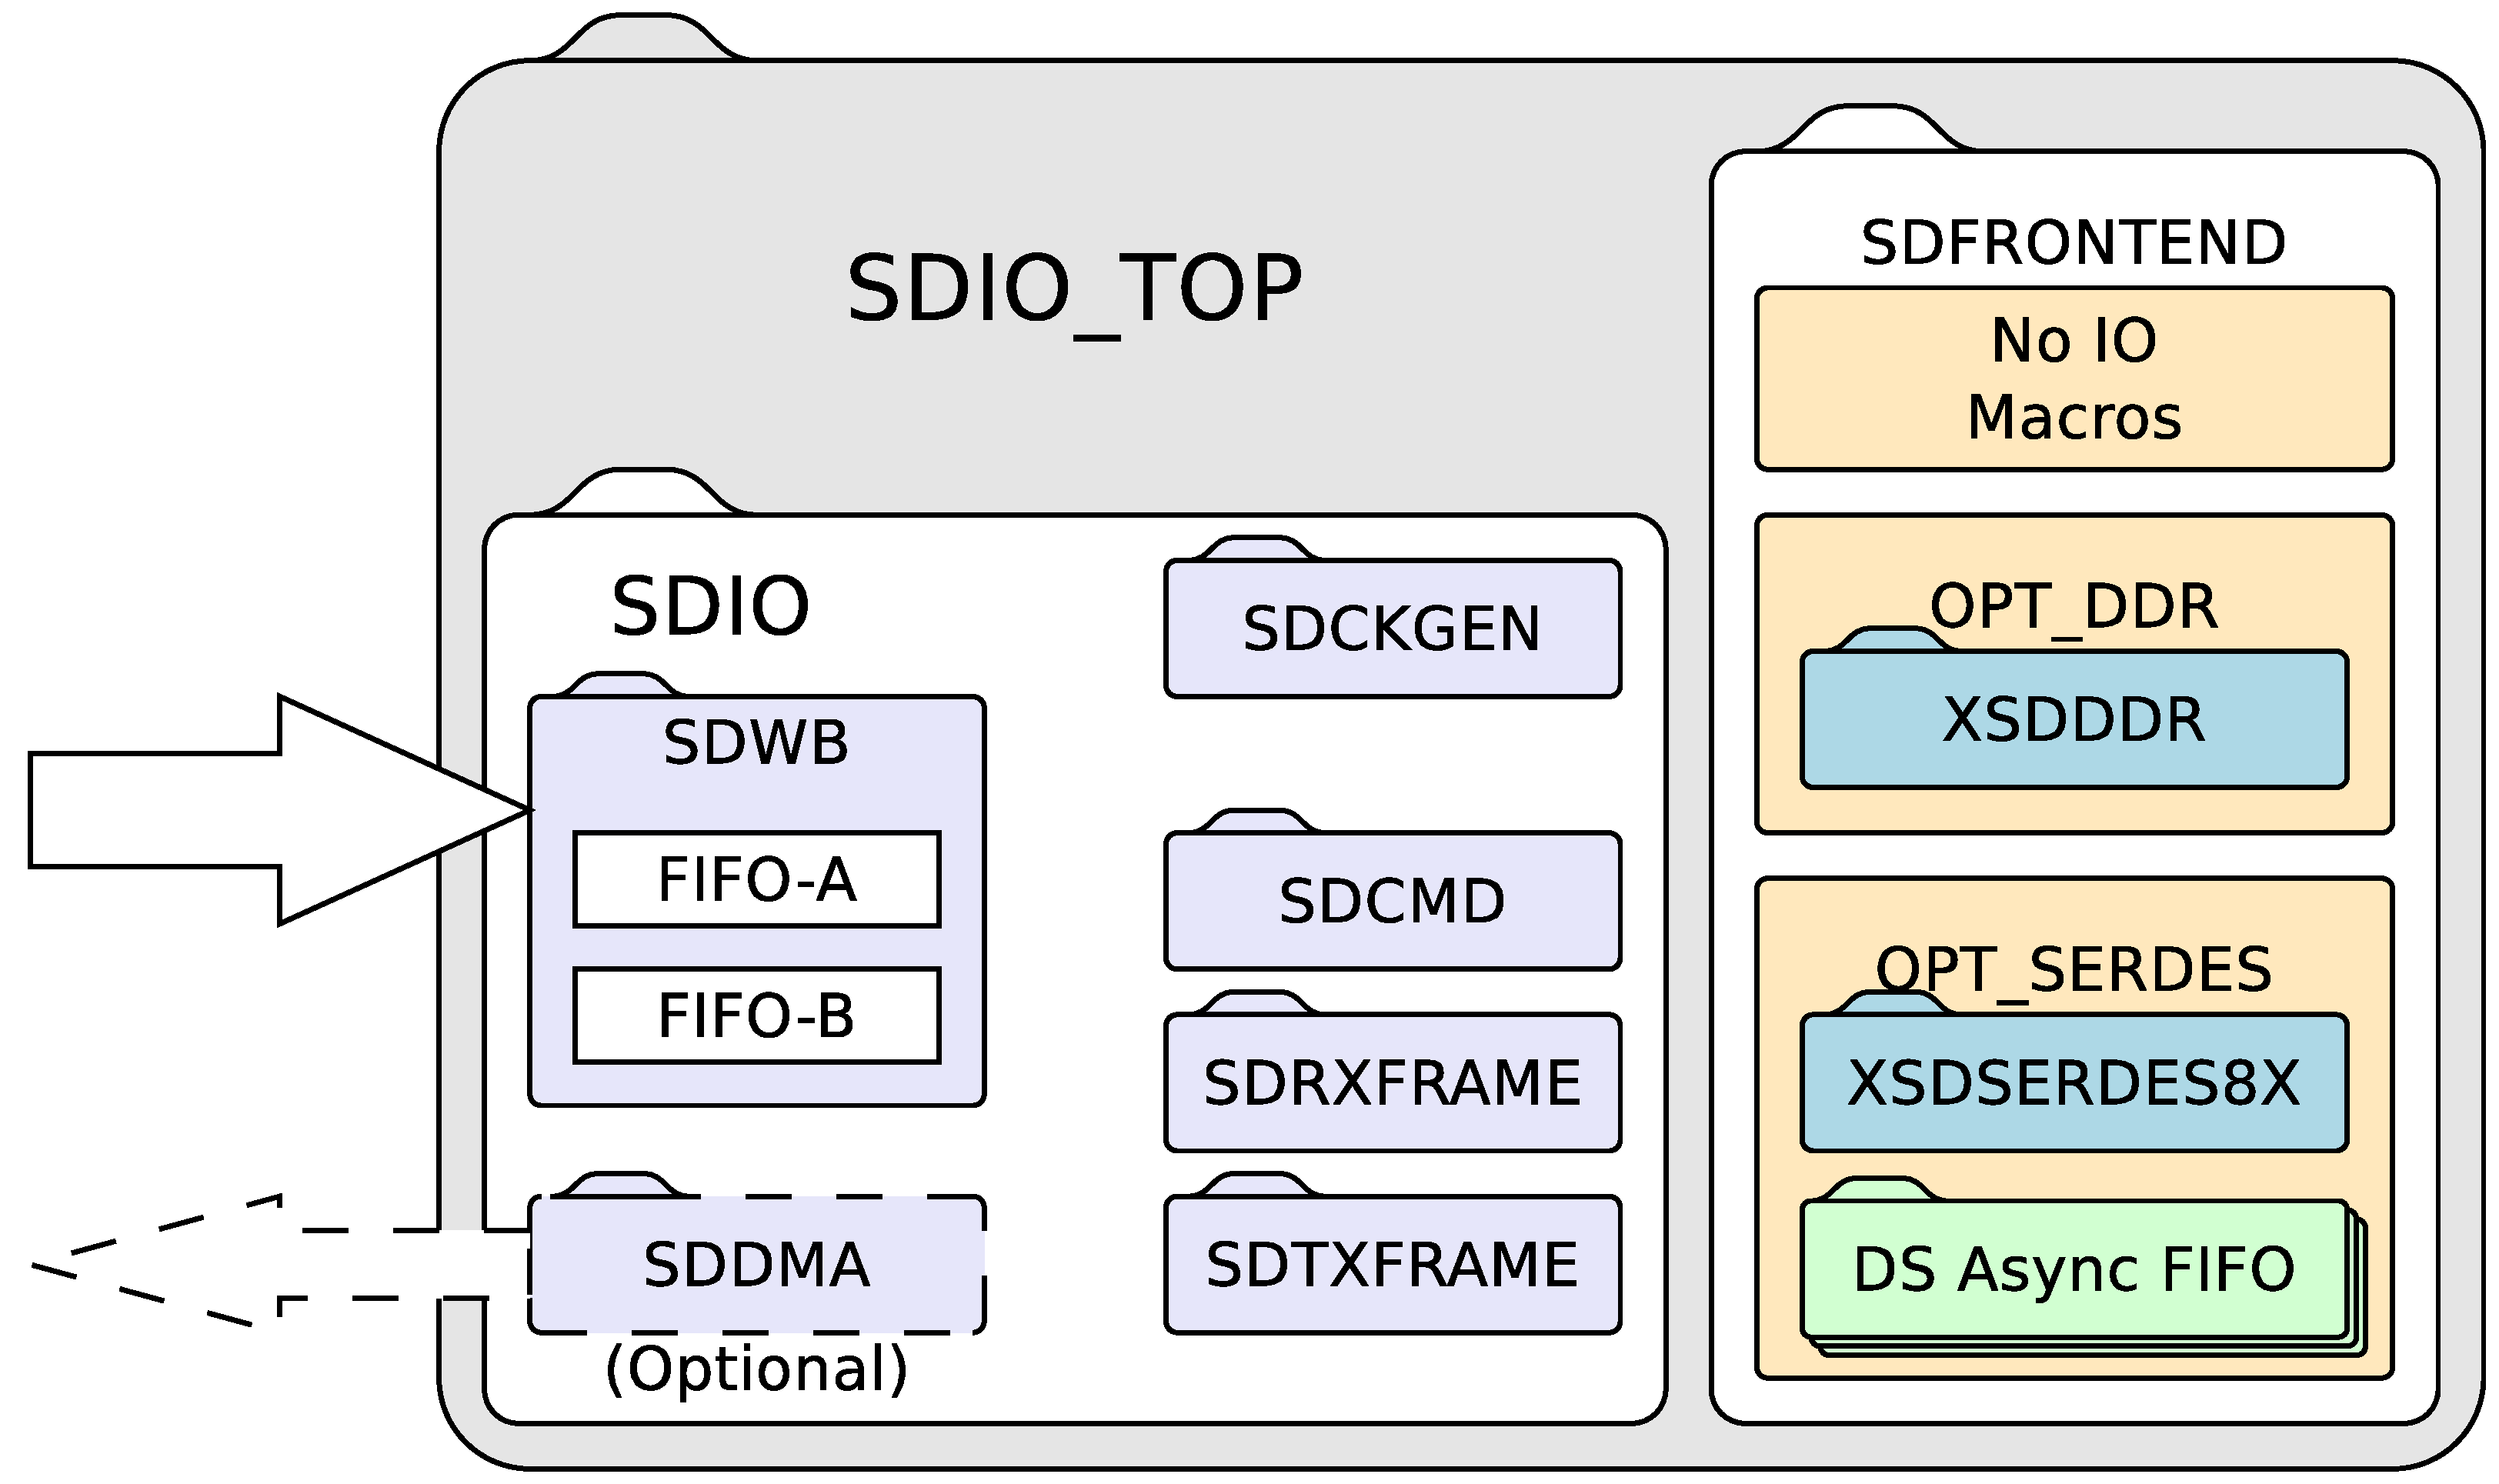
\includegraphics[height=2.5in]{gfx/sdioblocks.eps}
\caption{SDIO/eMMC Controller RTL Architecture}\label{fig:sdioblocks}
\end{center}\end{figure}
The design is broken up into two parts at the top level: a hardware independent,
all digital logic component whose top level is {\tt sdio.v}, and a hardware
dependent front end component whose top level is found in {\tt sdfrontend.v}.

The core controller, found in {\tt sdio.v}, itself is composed of five separate
components.  The first, {\tt sdwb.v}, is the controller.  This component is
a wishbone slave.  All user interaction goes through this controller.
Requests for transfers are made here.  Data to be transferred is stored here
in one of two FIFOs for transmission to the front end.  Data to be received
is stored here after reception, to be read out as it becomes available to the
CPU.

The controller maintains a register for configuring the front end.  This
register also controls the clock generator, {\tt sdckgen.v}.  This clock
generator is responsible for generating the clock used throughout the
system.  That clock is an 8-bit vector, allowing it to specify zero, one, or up
to two clock periods, each either aligned with or 90 degrees offset from the
data, per 8-bits.  This clock may also be divided to slower speeds as requested
by the user.  Finally, a user setting allows the clock to turn off when it isn't
being used, to save on interface power.  (Note that this only turns off the
IO clock, not any of the system clocks used throughout the design to clock
the logic within the design.)

Commands issued to the controller will be forwarded to the {\tt sdcmd.v}
module.  This module is responsible for all interactions taking place over
the CMD wire.  The module can generate 48-bit commands, beginning with a
start bit and ending with a CRC and a stop bit.  It can then recognize
either 48-bit or 136-bit command responses.  Responses are checked against
both the CRC and frame errors.  If the device fails to return a response
within a given timeout window, the response may also timeout with an error,
after which the command controller will no longer expect any response until
the next command is sent.

Fig.~\ref{fig:sdcmdflow}
\begin{figure}\begin{center}
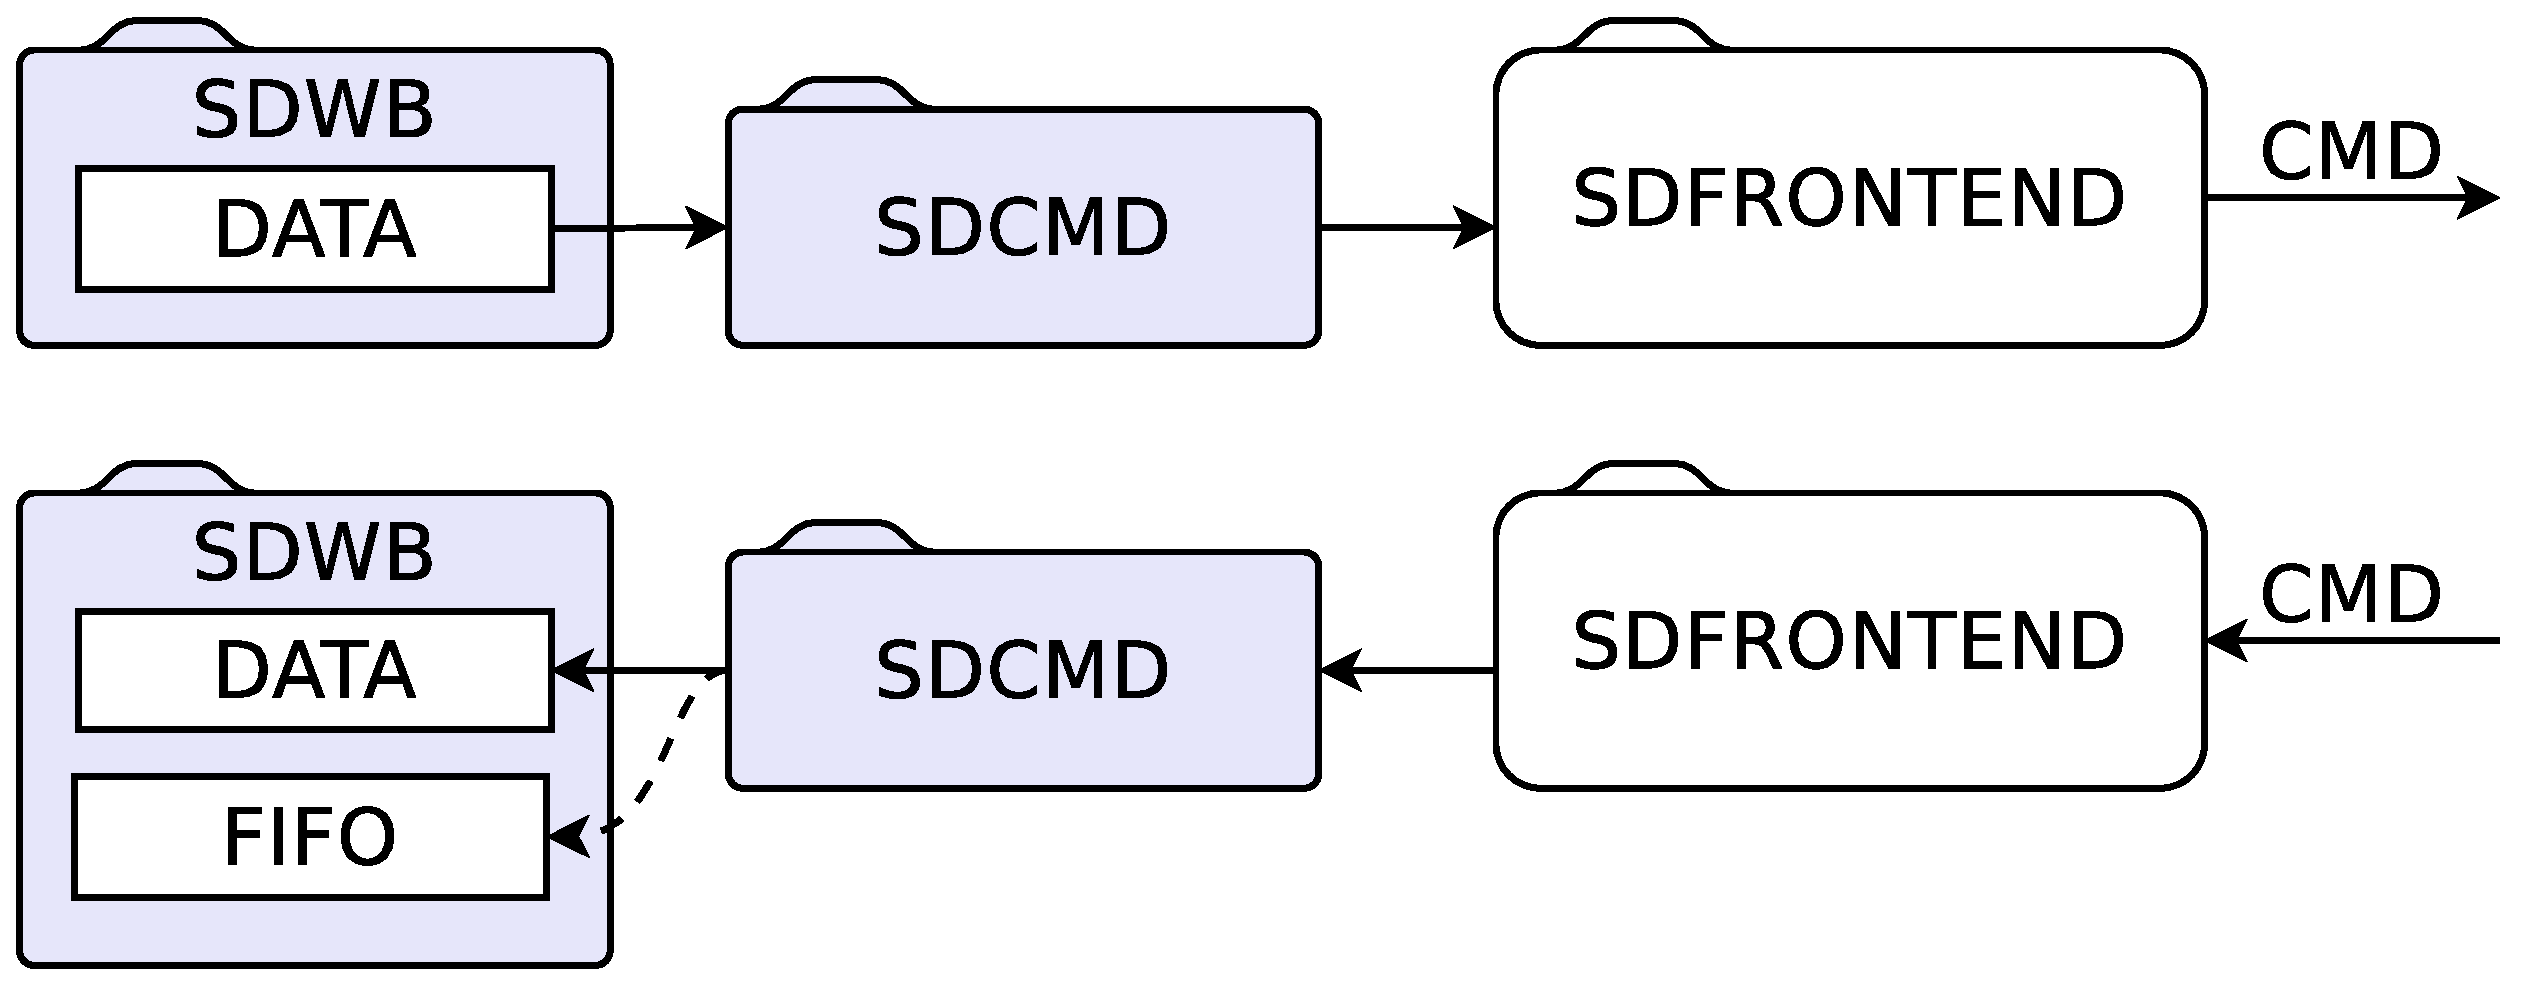
\includegraphics[width=5.0in]{gfx/sdiocmdflow.eps}
\caption{SDIO/eMMC CMD pin data flow}\label{fig:sdcmdflow}
\end{center}\end{figure}
shows both the basic command flow, and the two possible response flows.
For commands, a data register within {\tt sdwb.v} is first set, then the
command is issued.  The {\tt sdcmd.v} module organizes both into a 48-bit
word to be transmitted.  The {\tt sdcmd.v} module then looks for one of
two responses, either a 48--bit response which would place the 32-bit
argument back in a data register, or a 136--bit response which would be
placed into one of the two FIFOs in {\tt sdwb.v}.

One type of controller command is a memory command.  These commands send a
48-bit command to the device, followed by sending data to or receiving data
from the device.

The {\tt sdrxframe.v} component is activated when data is expected from the
device on the data wires.  It's purpose is to collect the data returned from
the front end controller, and reform that data into commands to write to
one of the FIFOs in {\tt sdwb.v}.  If a full frame, as defined by the
controller, is not received prior to a timeout, or if a CRC error is detected
within that frame, the receive component will report an error and give up
in order to wait for its next command.

Similarly, the {\tt sdtxframe.v} command is activated when data is to be
sent over the data wires to the device.  In this case, data flows from one
of the FIFOs in {\tt sdwb.v} to {\tt sdtxframe.v}, get formatted for the
front end to output, a start bit, CRC, and stop bit are added, and all get
sent to the front end.  This basic flow is shown in Fig.~\ref{fig:sdiotxflow}.
\begin{figure}\begin{center}
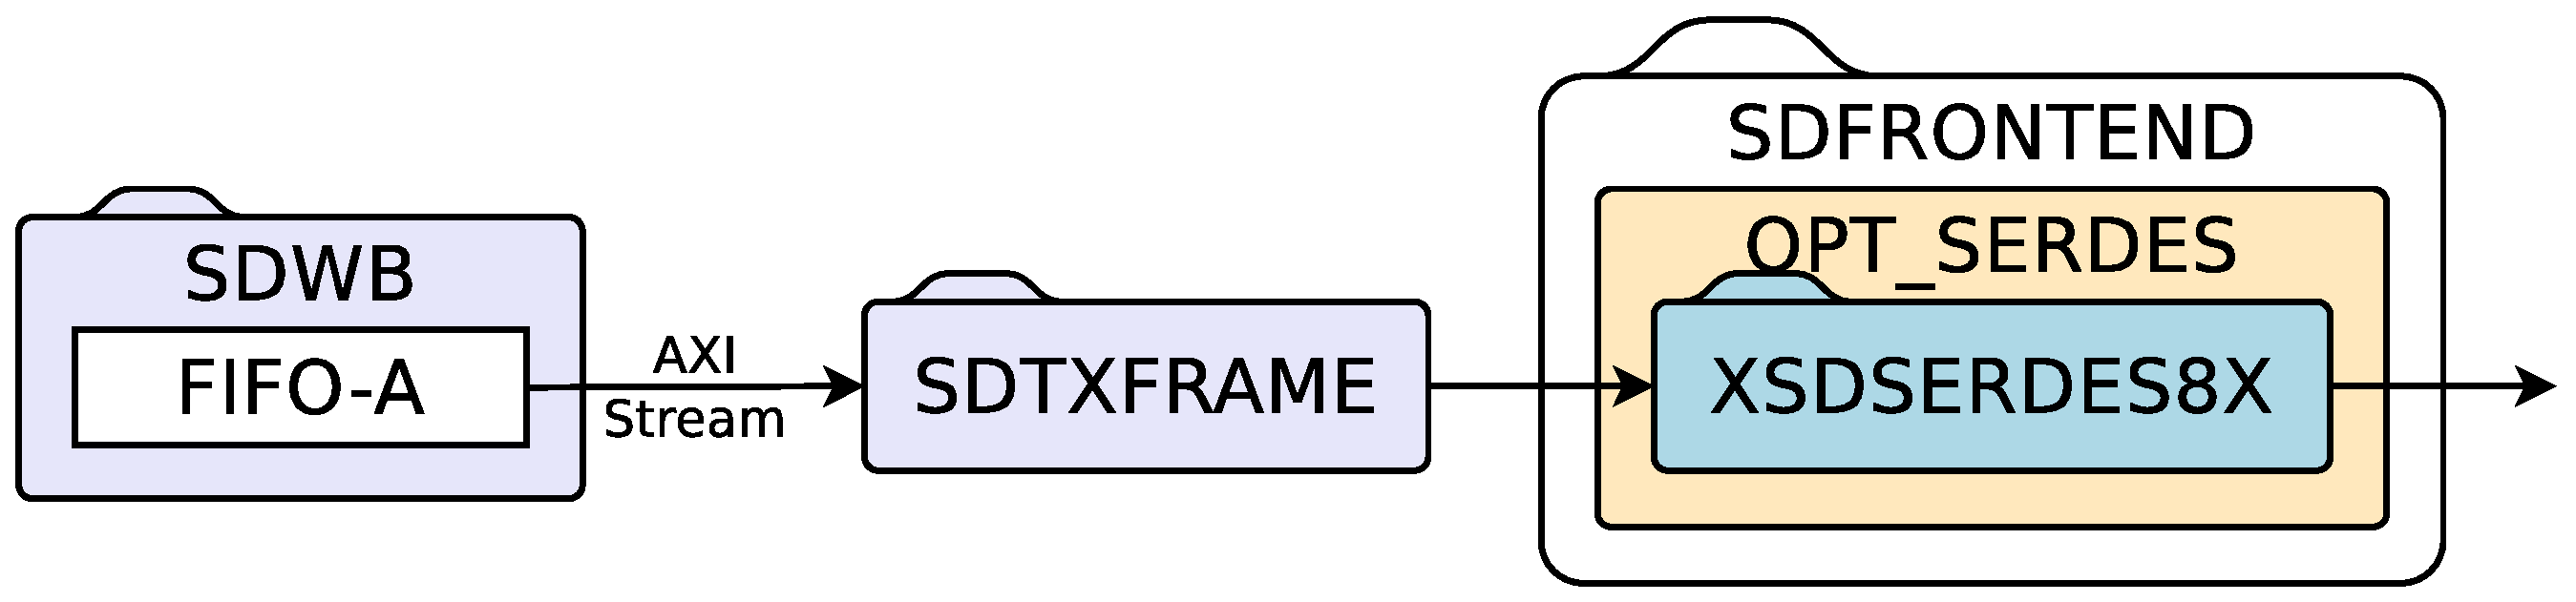
\includegraphics[width=5.0in]{gfx/sdiotxflow.eps}
\caption{SDIO/eMMC transmit data flow, to the device}\label{fig:sdiotxflow}
\end{center}\end{figure}

Let's now turn our attention to the device dependent front end.

The front end was initially defined for full IO support, all the way up to
HS400 and the eMMC data strobe.  Driven from a 100~MHz clock, this means that
this front end was designed to support up to two device clocks per 100~MHz
system clock, and to have data sent on each edge of these clocks.  This
forces a requirement of 4-data bits output per 100~MHz system clock cyle.
The clock, however, also needs to be (potentially) offset by 90~degrees from
that data.  As a result, all I/O using this particular front end capability,
called the {\tt OPT\_SERDES} capability in Fig.~\ref{fig:sdioblocks}, takes
place using Xilinx's 8:1 OSERDES elements.  Incoming bits are either sent
to an asynchronous FIFO, to support the eMMC data strobe, or they are
sampled via 1:8 ISERDES elements.  In the case of the ISERDES inputs, sample
timing is controlled via both the output clock rate, as well as a user
controlled digital delay, allowing sample alignment with clock precision
of one eighth of a system clock.  Hence, even without the full speed HS200
support, this subsample re-alignment may still be quite valuable when supporting
higher speeds.  All Xilinx specific SERDES interactions are captured in an
{\tt xsdserdes8x.v} module.

Logic resources throughout the design may be reduced, however, by switching
to a simpler front end architecture.  Two other architectures are available:
the {\tt OPT\_DDR} architecture and a plain architecture that doesn't use
any IO macros--save for the {\tt IOBUF} macro used for controlling any
tristate capabilities.

The {\tt OPT\_DDR} architecture is roughly the same as the {\tt OPT\_SERDES}
architecture, save the DDR IO elements are used to generate both clock and
data instead of the SERDES elements.  This should make it possible to drive
the IO pins at the full clock speed using SDR, or at half the clock speed
using DDR.  In this case, all Xilinx specific IDDR and ODDR interactions are
captured in an {\tt xsdddr.v} module.

The no macro architecture was built in order to support an architecture
where the {\tt SD\_CK} pin was routed through the Xilinx {\tt CCK} pin,
and hence through an {\tt STARTUPE2} primitive.  In this case, no IO macros
are available for controlling the clock, and all IOs are controlled directly
from logic.  The fastest clock this architecture can generate is half the
system clock rate.

These constitute the basic components of the controller, both hardware
independent and hardware dependent.

\section{Verification Architecture}\label{sec:arch-vip}

The verification architecutre is built around a model of the
downstream device.  One such model is shown in Fig.~\ref{fig:mdlsdio}.
\begin{figure}\begin{center}
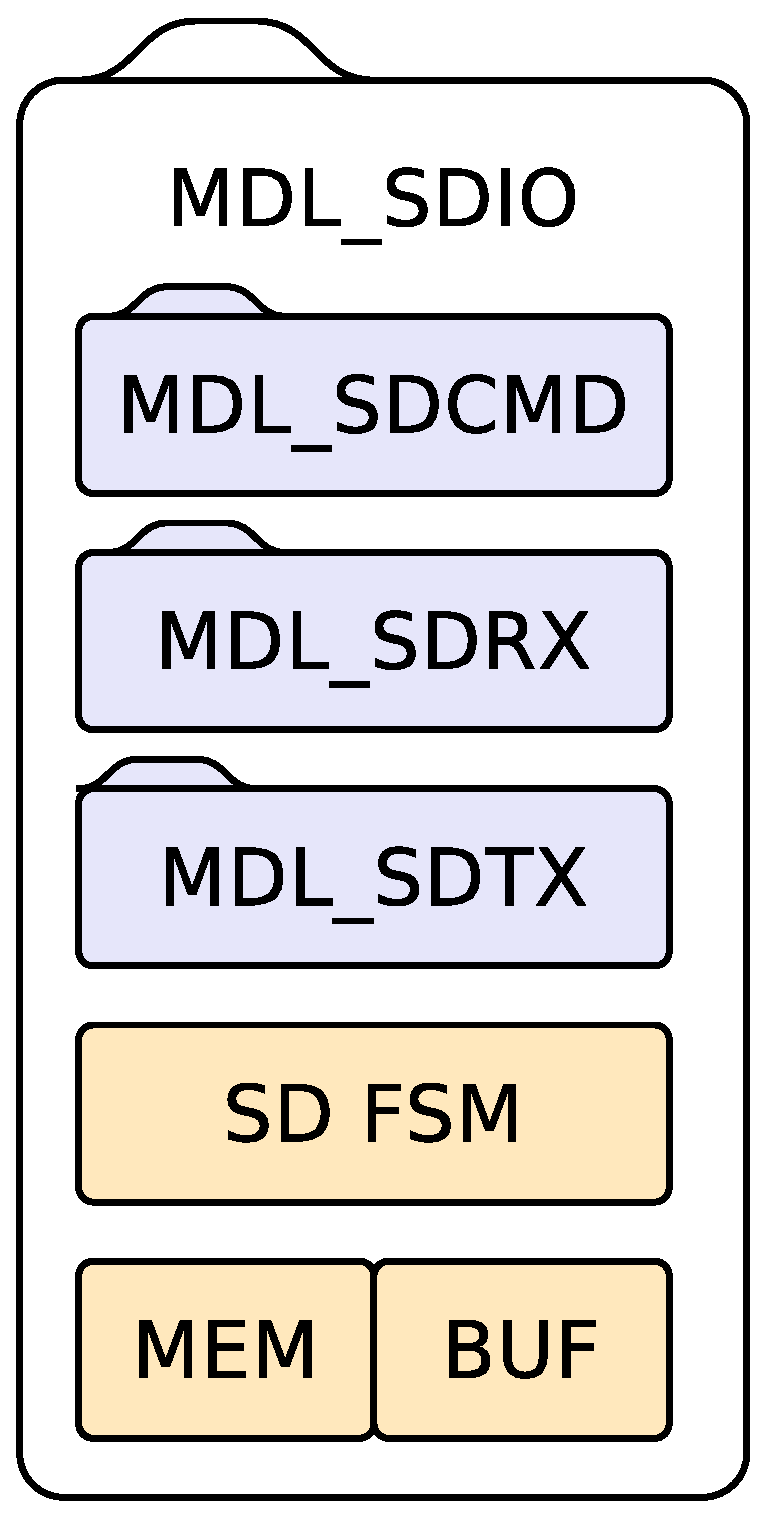
\includegraphics[height=2.5in]{gfx/mdlsdio.eps}
\caption{SDIO Verification IP}\label{fig:mdlsdio}
\end{center}\end{figure}
This Verification IP contains full featured submodules for handling the
command wire, receiving data, and transmitting data.  These three submodules
are designed to correspond to their host controller counterparts.  Further,
these three submodules have been built to be independent of whether the
controller is modeling an SDIO or an eMMC interface.

The smarts of this Verfication IP (VIP) are found in the finite state machine
(FSM) at the top level of {\tt mdl\_sdio.v}.  This machine respnds to commands,
and generates responses to them.  A data transfer buffer exists for sending
or receiving data across the interface.  A second memory within the VIP,
shown as {\tt MEM} in Fig.~\ref{fig:mdlsdio}, captures the persistent memory
found in the SDIO or eMMC device.

The entire Verilog test bench infrastructure is diagrammed in
Fig.~\ref{fig:vlogtb}.
\begin{figure}\begin{center}
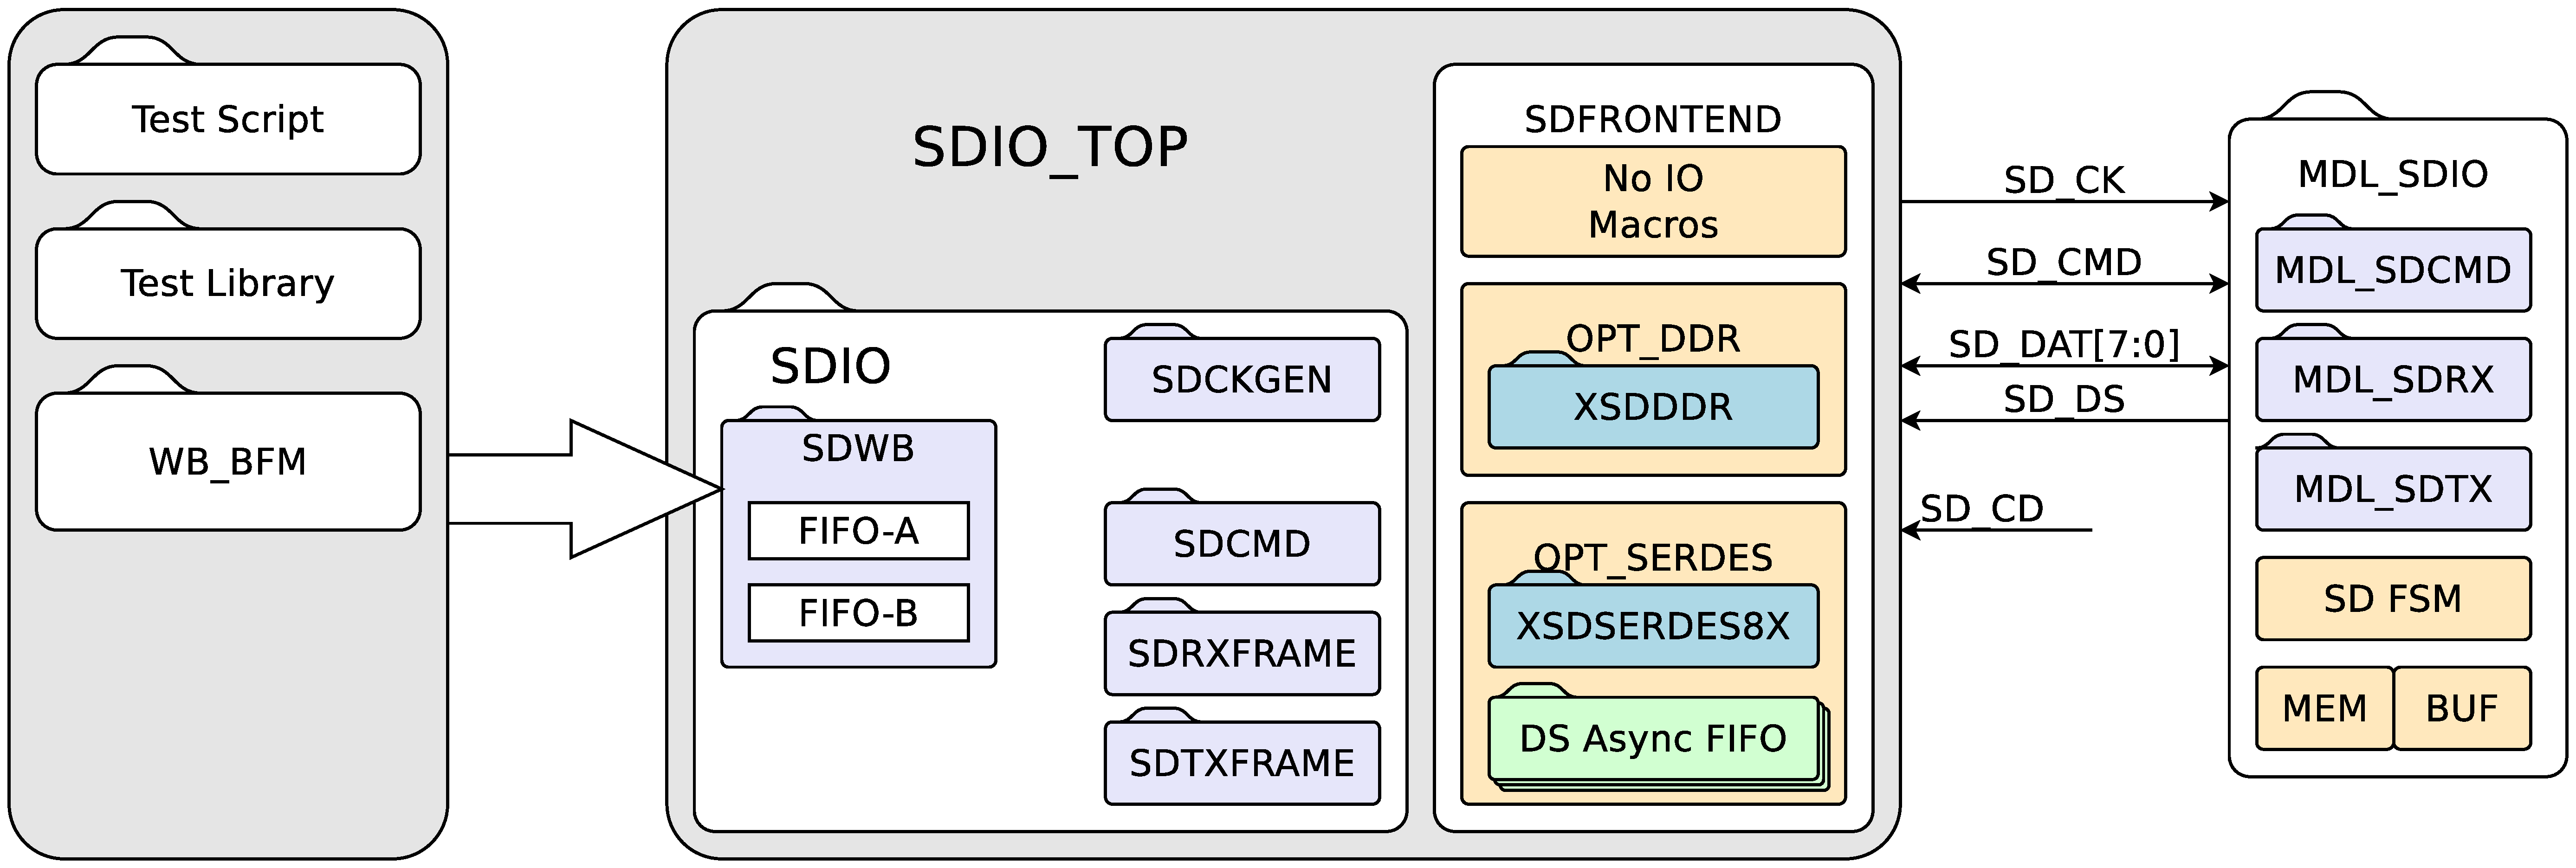
\includegraphics[width=5.0in]{gfx/vlogtb.eps}
\caption{All Verilog top-level model}\label{fig:vlogtb}
\end{center}\end{figure}
In this setup, a test script drives a Wishbone Bus Functional Model (BFM).
The BFM then drives the controller to interact with the VIP model.
What tests get accomplished at this point is dependent upon the test script.
A test library is available, for the purpose of defining common constants
and supporting common test script tasks.

A second test bench infrastructure, shown in Fig.~\ref{fig:cputb},
\begin{figure}\begin{center}
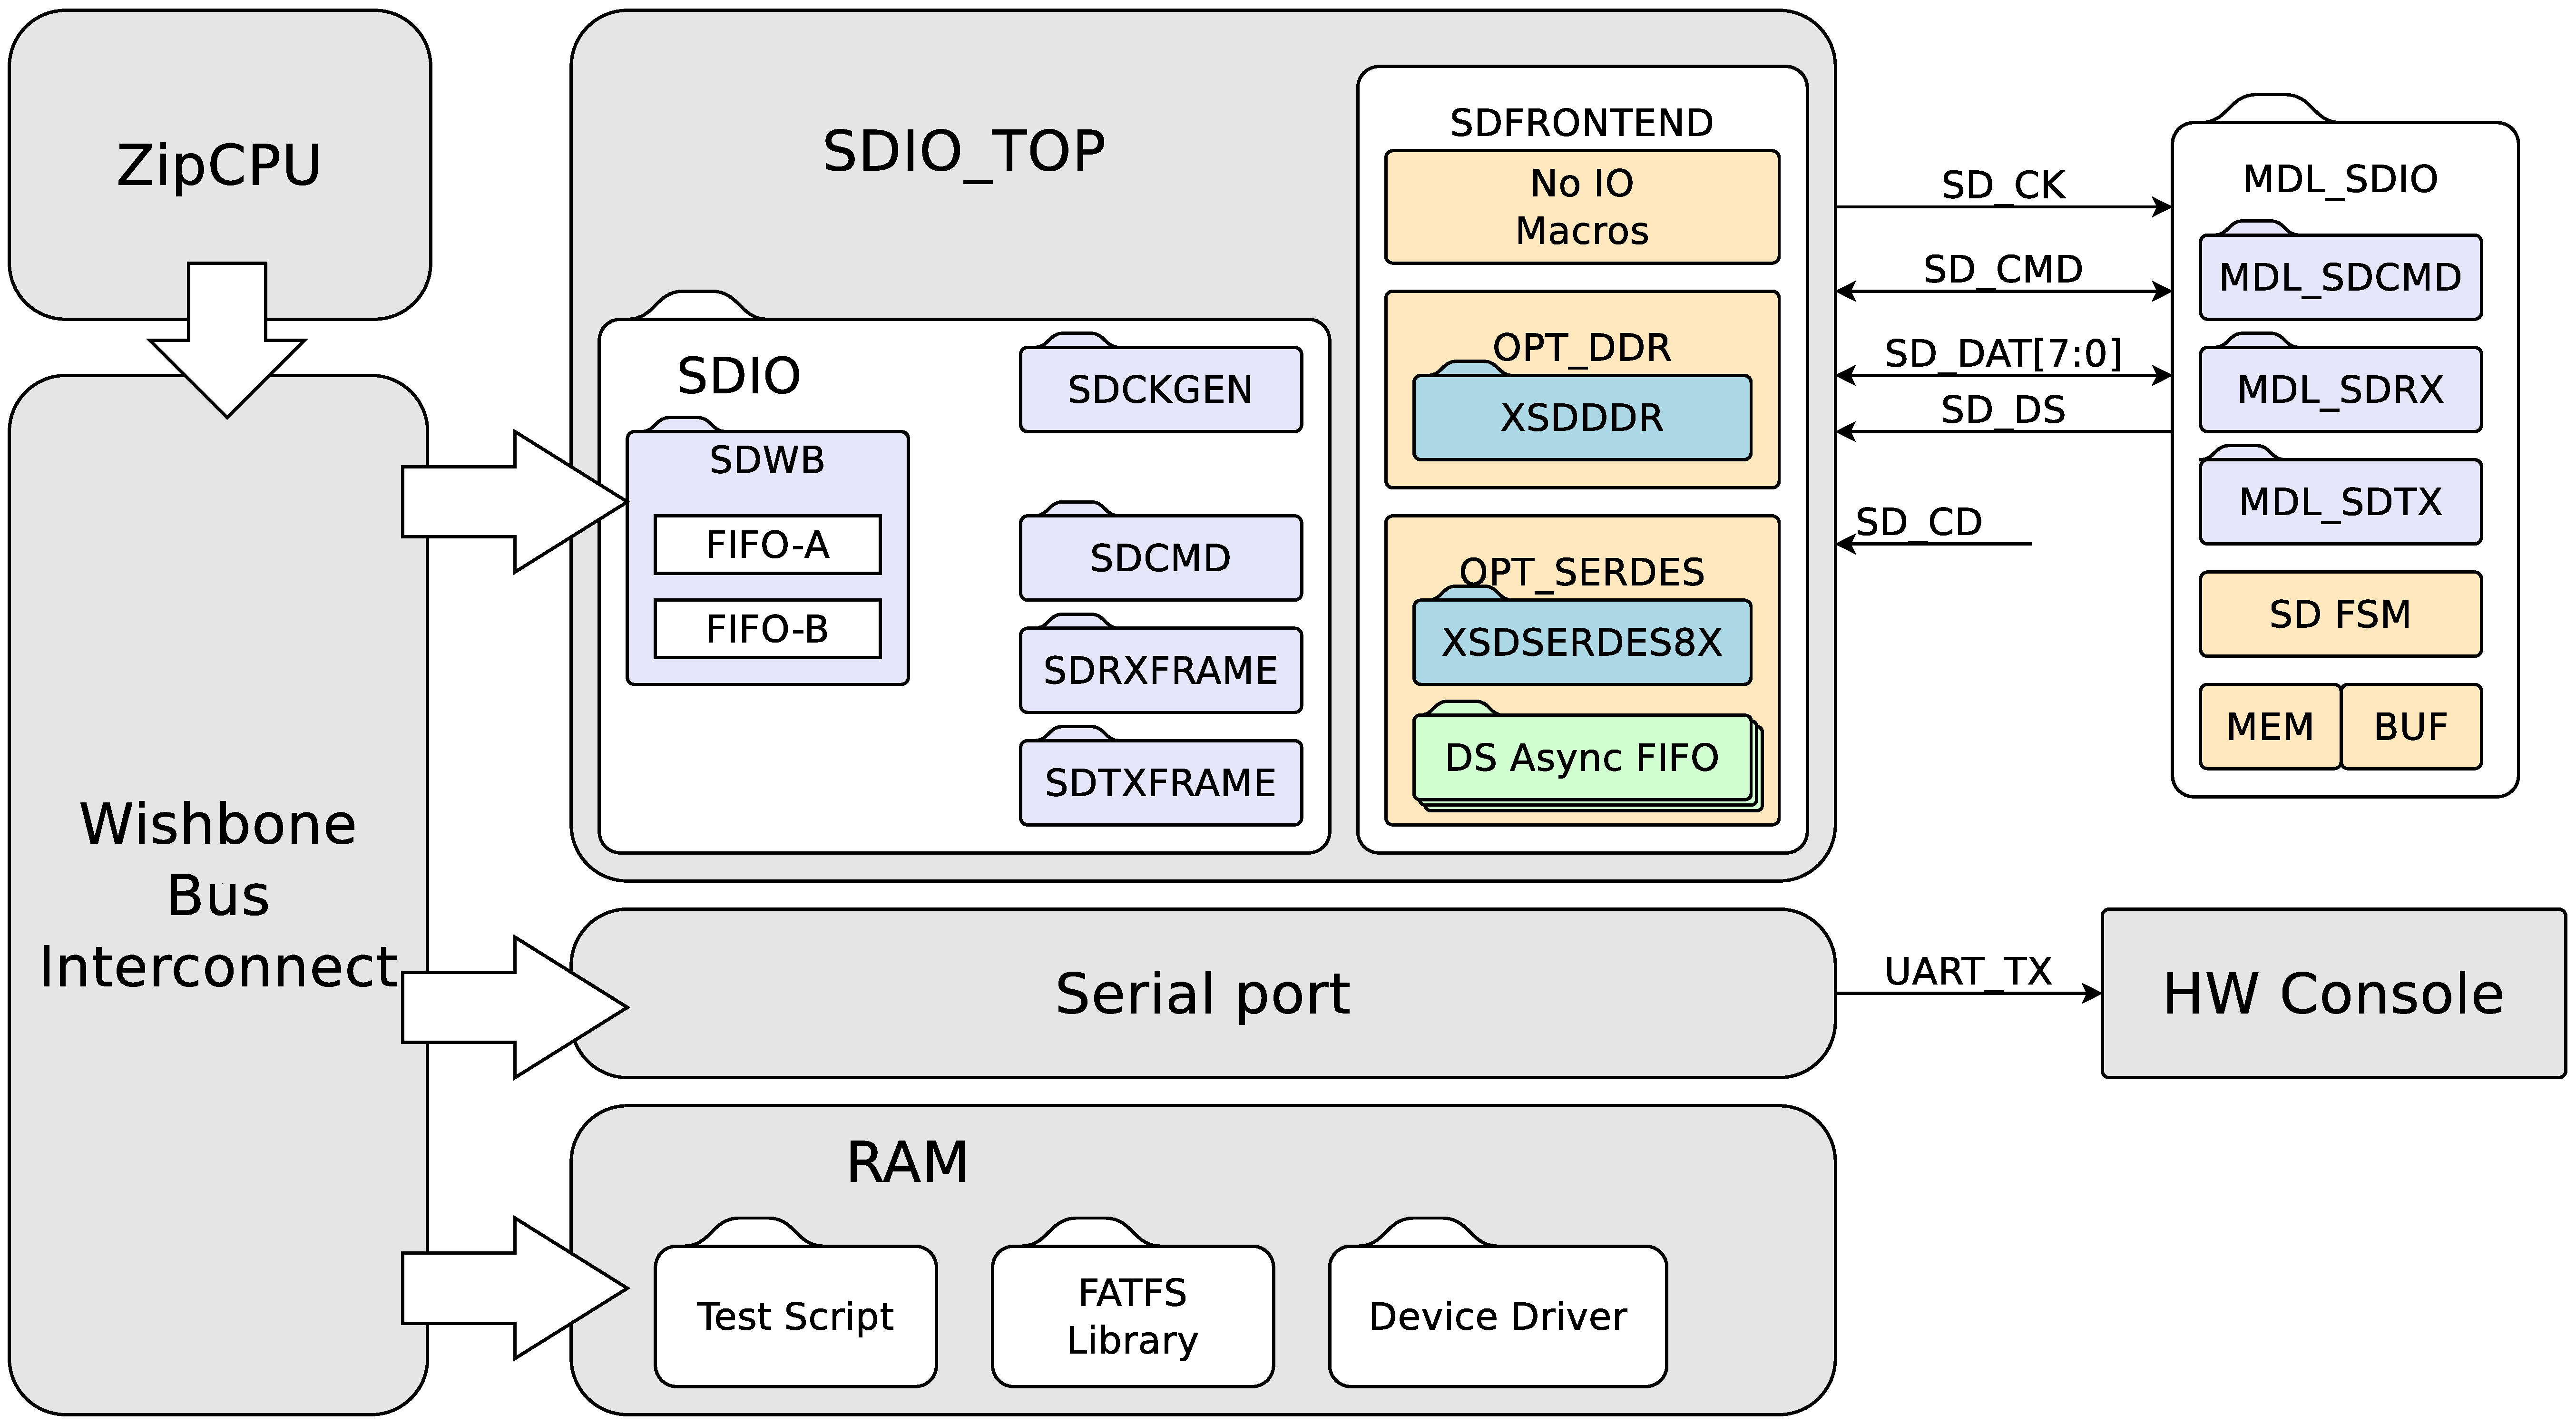
\includegraphics[width=5.0in]{gfx/cputb.eps}
\caption{All Verilog top-level model}\label{fig:cputb}
\end{center}\end{figure}
is also planned.  This infrastructure contains a soft--core ZipCPU,
serial console, and memory.  In this test architecture, the test script
exists as a software program supported by both the FATFS library and the
software driver.  The purpoes of this second infrastructure is to specifically
test and verify the software driver in its native (software) form, compiled
for and then running on a soft--core CPU.  In this case, that softcore CPU
will be the ZipCPU.

\section{Software Driver Architecture}\label{sec:arch-swdrvr}

At present, there exist three software drivers and one glue layer for each.
The three drivers are found in the {\tt sw/} directory.  These drivers are:
\begin{itemize}
\item {\tt sdspidrv.c}: A software driver for the SPI version of this
	controller.  The SPI version of this controller is described in the
	SDSPI user guide.
\item {\tt sdiodrv.c}: A software driver for the SDIO controller, described
	in this user guide.  This controller is designed to interact with
	an SD Card.
\item {\tt emmcdrv.c}: A software driver for the eMMC controller.  This is
	designed to interact with the same SDIO/eMMC controller discussed in
	this user guide.  However, the SDIO and eMMC protocols require different
	commands to interact with their respective devices.  As a result, the
	eMMC software driver differs significantly from the SDIO software
	driver.
\item {\tt diskiodrvr.h} provides a common definition of a device ``driver'',
	which can be used across all of the device drivers listed above.

	More on this in a moment.
\item {\tt diskio.c} is a shared/common dispatch glue layer.  Commands
	from the FATFS subsystem naturally land here, where they are then
	dispatched to the appropriate controller.
\end{itemize}

Put together, this IO subsystem has the various layers shown in
Fig.~\ref{fig:swlayers}.
\begin{figure}\begin{center}
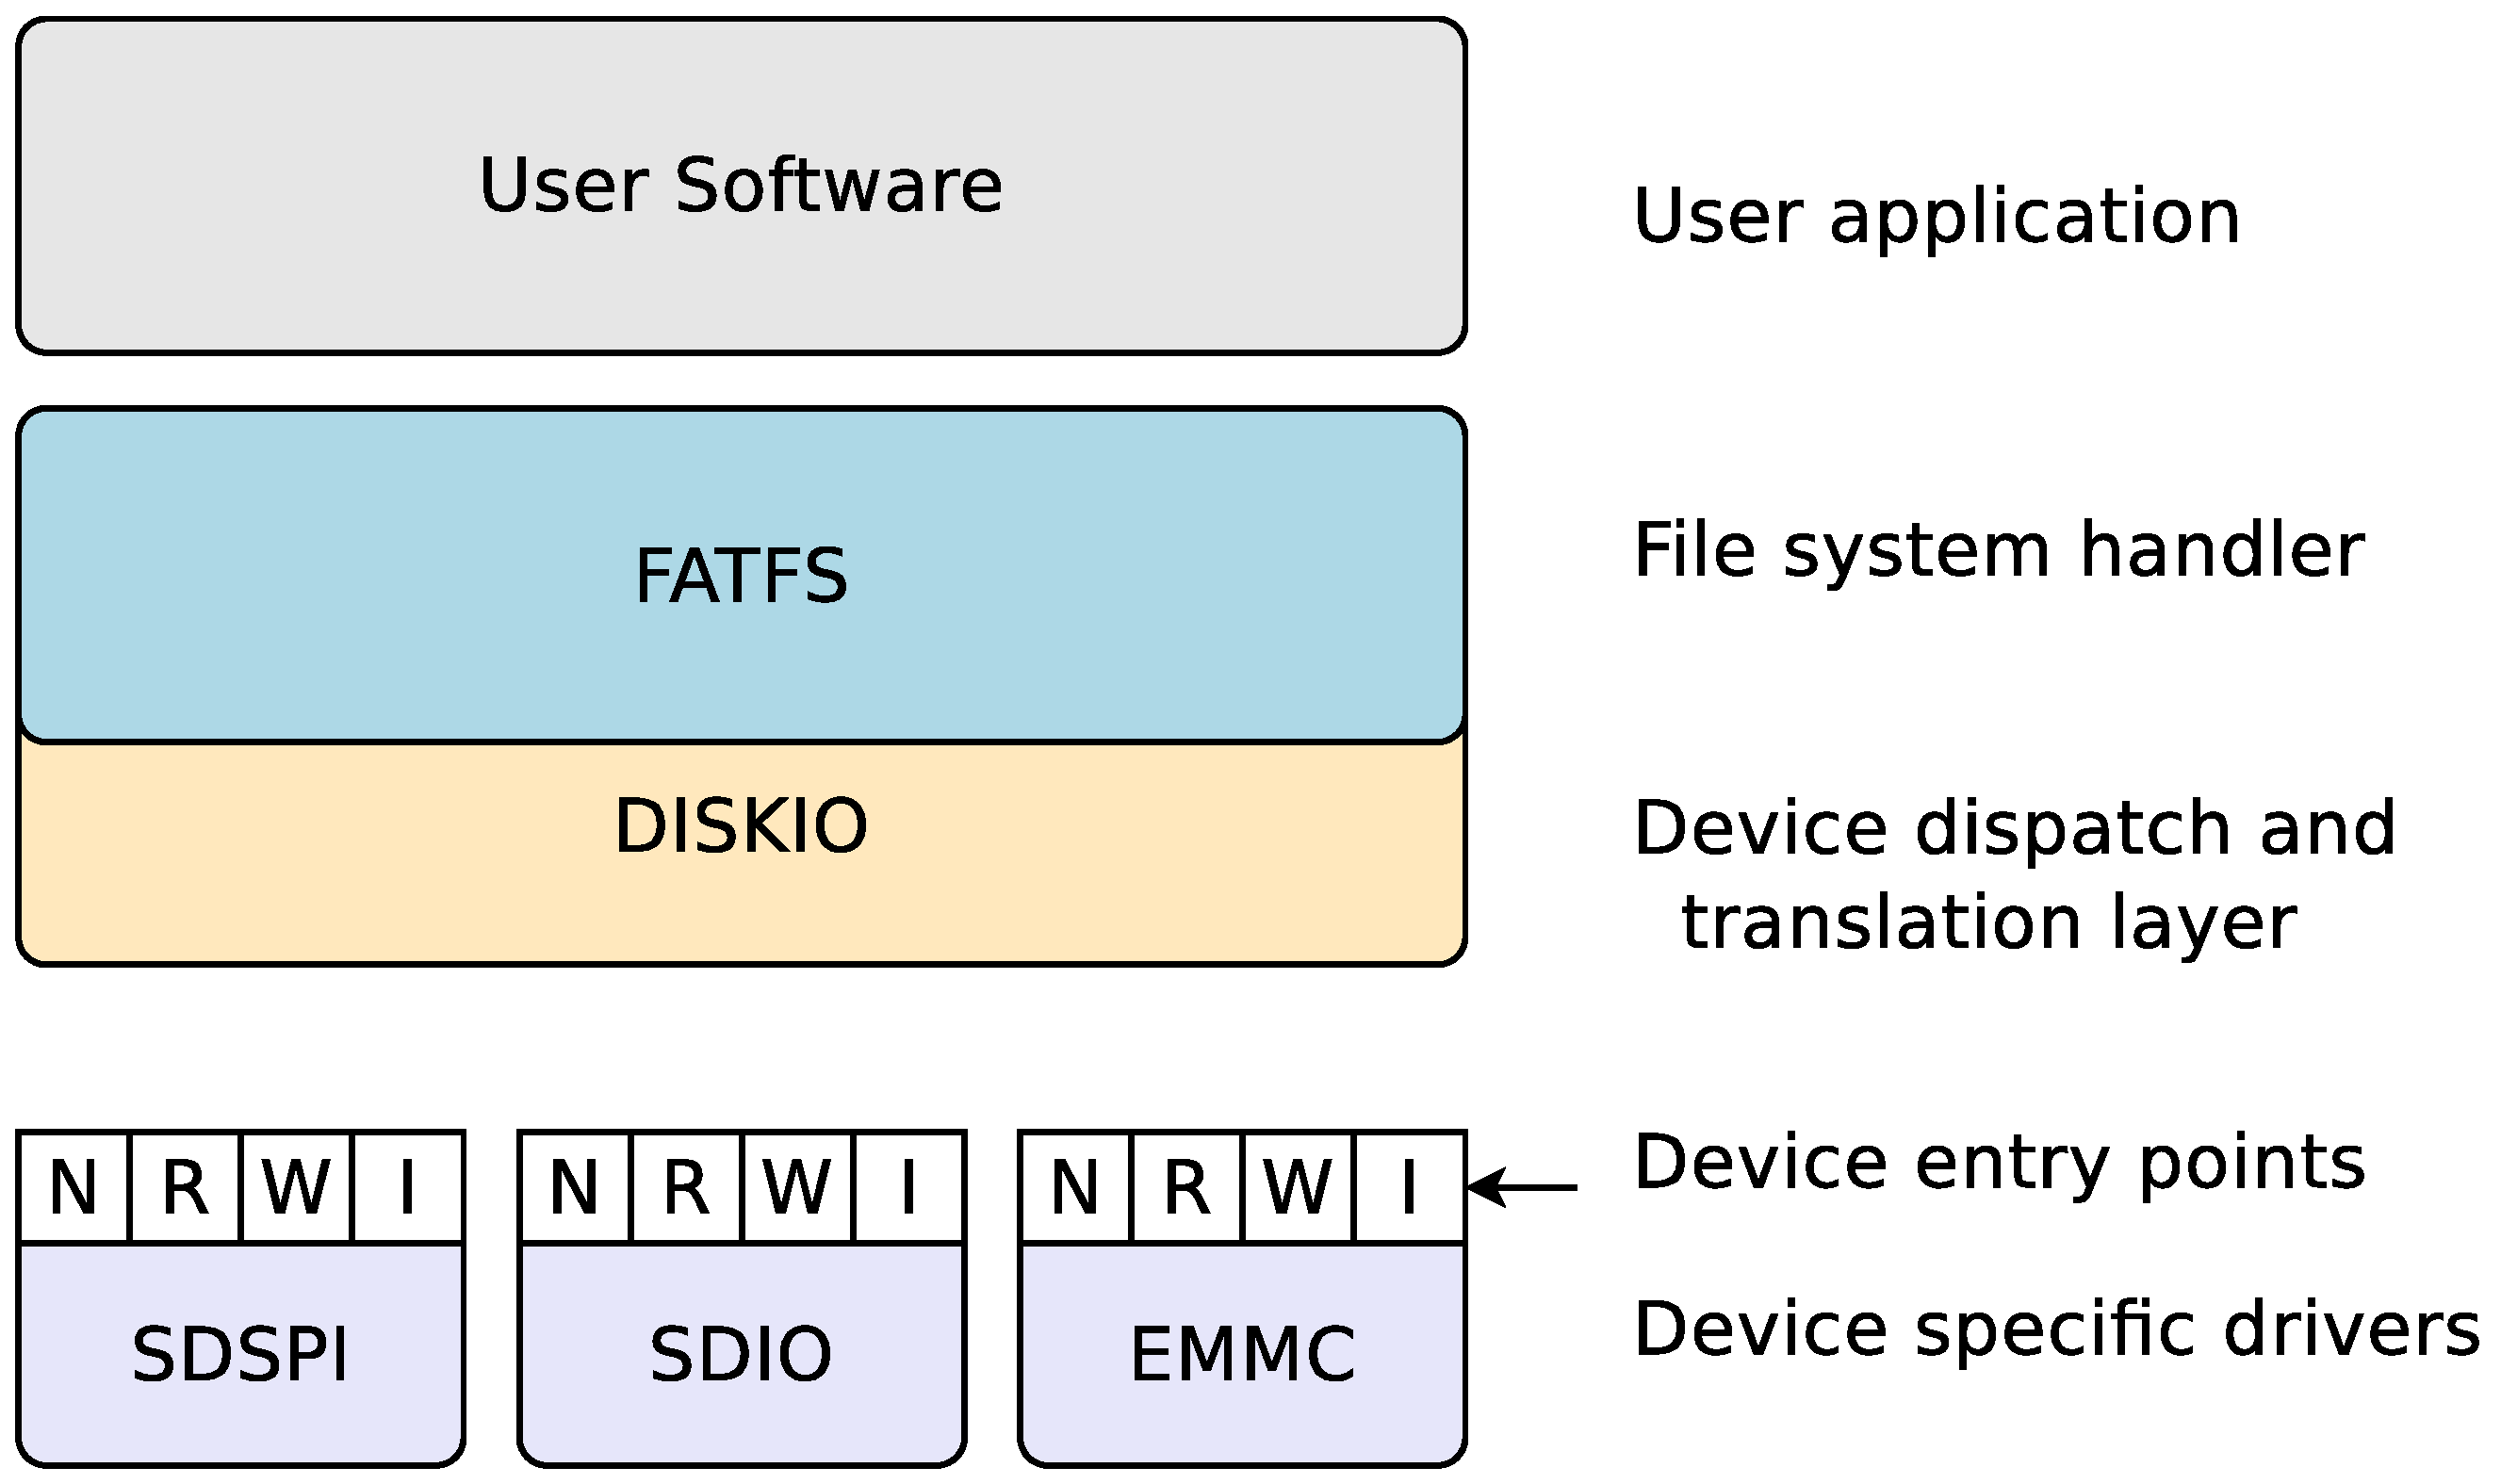
\includegraphics[height=2.5in]{gfx/swlayers.eps}
\caption{Software Stack}\label{fig:swlayers}
\end{center}\end{figure}
User software interacts with the FATFS layer.  FATFS then interacts with the
device dispatch layer.  The device dispatch layer then instantiates and
interacts with one (or more) of the device drivers beneath it.

Each device driver has four entry points--``methods'' in Object Oriented
terminology.  The first method is used to initialize the driver and set up
its data structures.  After that, there are methods for reading and writing.
Finally, there's an IOCTL method which can be used for other tasks such as
querying the size of the device or the size of a data block.

%% }}}
\chapter{Operation}\label{ch:ops}
%% {{{
At its most basic level, interacting with the controller simply involves
configuring the PHY, setting the data you wish to send, and then sending a
command to the controller.  This needs to take place, however, in many
different contexts.  Some commands don't expect responses, whereas others
return 48 or even 136--bits.  Some commands include data transmission,
whereas others do not.  This section therefore walks through several
examples of commands, illustrating the range of commands and responses
that can be issued using this controller.

\section{Initial PHY setup}
%% {{{
The first step to any operation is to make sure that the PHY register
is appropriately set up for the clock speed desired, the transfer rate
desired, and whether or not the design will be using open--drain or push--pull
IOs.  Any changes made to this register will be applied immediately, save
for any changes to the clock rate.  Clock rate changes will take place starting
at the top of the next clock cycle.  Hence, once a clock rate change has been
made, it makes sense to wait until the current clock matches the requested
clock rate.

The following, for example, will set up a 100~kHz clock rate using open--drain
IOs and 512~byte sector sizes.  This is appropriate for beginning communication
with the device.

\begin{zCpp}
	const	SDIOCK_100KHZ = 0x000000fc,
		SPEED_SLOW    = SDIOCK_100KHZ,
		SPEED_512B    = 0x09000000;

	_sdio->sd_phy = SPEED_SLOW | SECTOR_512B;
	while(SPEED_SLOW != (_sdio->sd_phy & 0x0ff))
		;
\end{zCpp}
%% }}}
\section{GO IDLE: Commands that don't get responses}
%% {{{
Sending a command to the device is as easy as setting the commands 32'bit
data, and then writing the appropriate command to the command register.
All command writes set bits [7:6] to 2'b01.  Non-command writes will set these
bits to something different.  At the same time you write a command to the
controller, you'll also want to tell the controller what type of
response to expect--whether to expect no response at all, an 48-bit (R1)
response, or a 136-bit (R2) response.

When issuing a command, you also want to be aware of the error bit.  If the
error bit gets set, no commands will be accepted until the error bit is cleared.
Hence, you'll want to clear the error bit at the beginning of any command
sequence, and check it when you are done to see where any error took place.

Finally, in the case of the first command used when interacting with a device,
you'll want to clear the controller's card-removed bit.  You can then check
this bit later, at your convenience, to know if the card has ever been removed
and (if so) if you need to start your initialization sequence again from
the {\tt SEND\_GO\_IDLE} command.

Put together, this would look like:
\begin{zCpp}
	const	SDIO_REMOVED = 0x00040000,
		SDIO_ERR     = 0x00008000,
		SDIO_RNONE   = 0x00000000,
		SDIO_CMD     = 0x00000040;

	_sdio->sd_data = 0;
	_sdio->sd_cmd  = SDIO_REMOVED | SDIO_CMD | SDIO_RNONE | SDIO_ERR;
\end{zCpp}

The next step is to wait for the command to complete.  This can be done either
by polling the controller,
\begin{zCpp}
	const	SDIO_REMOVED = 0x00104800;

	unsigned	st;

	st = _sdio->sd_cmd;
	while(st & SDIO_BUSY)
		st = _sdio->sd_cmd;
\end{zCpp}
or by waiting for a controller interrupt.
\begin{zCpp}
	// SDIO_INT is the interrupt number assigned to the
	// design.  It's set external to the controller.
	unsigned	st;

	st = _sdio->sd_cmd;
	while(st & SDIO_BUSY) {
		CLEAR_INT(SDIO_INT);
		WAIT_INT(SDIO_INT);
	}
\end{zCpp}

%% }}}
\section{SEND IF COND: R1 commands}
%% {{{
The next type of command the controller understands are what are called
R1 commands.  These are commands that expect a 48-bit response--whether
or not that response truly contains an R1 register or any other register.

The first R1 command in the startup script is the SEND IF COND command, also
known as CMD8.  This command requires a special argument.  We'll allow that
argument to arrive via the variable {\tt ifcond}.  This variable is first
placed in the {\tt sd\_data} register, and then the command is issued.

\begin{zCpp}
	const	SDIO_R1      = 0x00000100,
		SDIO_READREG = SDIO_R1 | SDIO_CMD;

	_sdio->sd_data = ifcond;
	_sdio->sd_cmd = SDIO_READREG+8;

	wait_while_busy();
\end{zCpp}

Once the command returns, the first 8-bits of the 48-bit return may be
read from the {\tt sd\_cmd} register.  If the protocol has been followed and
the device has returned a value, then bits [7:6] of this register will now
be zero.  The next 32-bits may be read from the {\tt sd\_data} register, to
know how the device has responded.  The last 8-bits, both CRC and stop bit,
are not returned.  Instead, the error bit and error code may be checked
to know if the CRC is correct and the stop bit valid.

%% }}}
\section{ALL SEND CID: R2 commands}
%% {{{
The last type of command is the R2 command.  These commands read 136-bits
from the device.  The first 8-bits of these are read into the command register,
as with the R1 commands.  However, the next 128-bits will not fit into the
data register.  Instead, they are returned into one of the two FIFOs.

Sending such a command follows the same script as before.  The difference is
that we could now specify, in our command, which FIFO to write the results into.
We'll use FIFO A, the first FIFO, which is the default for this example.

\begin{zCpp}
	const	SDIO_R2      = 0x00000200,
		SDIO_READREG = SDIO_R2 | SDIO_CMD;

	_sdio->sd_data = 0;
	_sdio->sd_cmd = (SDIO_ERR|SDIO_READR2) + 2;

	wait_while_busy();
\end{zCpp}

If this particular command works, it is likely to set the CRC error bit.
This is normal for a CMD2, although not so normal for other commands.

Once the command completes, the CID register can be read from the FIFO
32-bits at a time.

\begin{zCpp}
	unsigned	d_CID[4];

	d_CID[0] = _sdio->sd_fifa;
	d_CID[1] = _sdio->sd_fifa;
	d_CID[2] = _sdio->sd_fifa;
	d_CID[3] = _sdio->sd_fifa;
\end{zCpp}

If the controller has been configured for big--endian operation, then
the MSB byte of each FIFO result will be the first byte read from the
device.

The {\tt d\_CID} values may then be decoded and processed by the software
driver.
%% }}}
\section{Adjusting the PHY}
%% {{{
Once any cards have been properly enumerated, the PHY may be adjusted
for higher speed.  The first speed change below simply changes the clock
speed to 25MHz, and the IOs from open--drain to push--pull.

\begin{zCpp}
	const	SDIOCK_25MHZ = 0x00000003,
		SPEED_512B   = 0x09000000;

	_sdio->sd_phy = SECTOR_512B | SDIOCK_25MHZ | SDIO_PUSHPULL;
	while(SDIOCK_25MHz != (_sdio->sd_phy & 0x0ff))
		; // Wait for the clock change
\end{zCpp}

A later PHY adjustment might even include switching to 4--bit data mode.

\begin{zCpp}
	const	SDIO_W4 = 0x00000400;

	_sdio->sd_phy = SECTOR_512B | SDIOCK_25MHZ | SDIO_PUSHPULL
				| SDIO_W4;
\end{zCpp}

In this final example, we don't need to wait for the change to take place.
The interface was already idle, so it took place immediately.
%% }}}
\section{Reading a sector}
%% {{{
Once the SD card has been set up, the next step may be to read a sector
of data.  In general, this is as simple as enabling the FIFO when issuing
the command, and then reading the data from it once the command has been
complete.

The SDIO driver first, however, checks whether or not the card has been
removed.  This is appropriate, lest the card has been swapped unbeknownst
to the controller.
\begin{zCpp}
	if _sdio->sd_cmd & SDIO_REMOVED)
		return CARD_REMOVED_ERR;
\end{zCpp}

If the card has not been removed, then we can issue a command to read a
block.  This involves setting the {\tt SDIO\_MEM} bit and (potentially) the
FIFO bit to select which FIFO we are interested in.
\begin{zCpp}
	const	SDIO_MEM     = 0x00000800,
		SDIO_READBLK = (SDIO_CMD|SDIO_R1|SDIO_MEM)+17;

	_sdio->sd_data = sector;
	_sdio->sd_cmd = SDIO_READBLK;

	wait_while_busy();
\end{zCpp}

Once the read completes, we can check for any errors.

Assuming the read completed without error, we can then read the data back
out of the controller.

\begin{zCpp}
	for(int k=0; k<512/sizeof(uint32_t); k++)
		buf[k] = _sdio->sd_fifa;
\end{zCpp}

Note that the FIFO's are always 32-bit aligned.  Whether or not the buffer
is aligned, or whether or not the CPU supports unaigned accesses in the
case where it isn't, aren't controller issues.

The ZipCPU's DMA may also be used to read from this controller if desired
for higher speed.
%% }}}
\section{Writing a sector}
%% {{{
Writing a sector to the device is very similar to reading, however, there
are a few minor key differences.  The first key difference is that the memory
needs to be loaded into the FIFO first, before it can be sent to the device.
\begin{zCpp}
	for(int k=0; k<512/sizeof(uint32_t); k++)
		_sdio->sd_fifa = buf[k];
\end{zCpp}

The second key difference is that the controller doesn't know when to write
to the device or when to read from it.  In general, the controller doesn't
know the meanings of any of the commands.  Therefore, if a command needs to
use the FIFOs, the controller needs to be told.  Likewise, if the data is
suppoesd to flow from the FIFO to the device instead of from the device to
the FIFO, the controller also needs to be told.  For this reason, a separate
bit needs to be set in addition to the previous ones--one to indicate that
this is a write and not a read.

\begin{zCpp}
	const	SDIO_WRITE    = 0x00000400,
		SDIO_WRITEBLK = (SDIO_CMD | SDIO_R1 | SDIO_ERR
				| SDIO_WRITE | SDIO_MEM) + 24;

	_sdio->sd_data = sector;
	_sdio->sd_cmd  = SDIO_WRITEBLK;

	wait_while_busy();
\end{zCpp}
%% }}}
\section{Writing multiple sectors}
%% {{{
Writing multiple sectors to the device is very similar to writing a single
sector.  Indeed, the instructions for writing the first sector are identical,
save that the command is now a CMD25 instead of a CMD24.  Things become
different when it comes to writing subsequent sectors, and then when it comes
to ending transmission.

Let's walk through these changes one by one.

The first change is that we don't initially wait for the write to complete.

\begin{zCpp}
	const	SDIO_FIFO  = 0x00001000;

	_sdio->sd_data = sector;
	_sdio->sd_cmd  = (SDIO_CMD | SDIO_R1 | SDIO_ERR
				| SDIO_WRITE | SDIO_MEM) + 25;
\end{zCpp}

Instead, we load a second sector into the FIFO.  In general, we'll alternate
which FIFO we use.

\begin{zCpp}
	unsigned *src = &buf[s*512];

	if (s&1) {
		for(int w=0; w<512/sizeof(uint32_t); w++)
			_sdio->sd_fifb = src[w];
	} else {
		for(int w=0; w<512/sizeof(uint32_t); w++)
			_sdio->sd_fifa = src[w];
	}
\end{zCpp}

Once the second sector has been transferred to FIFO memory, we can then wait
for the current write transaction to complete and issue a new write request
for the next sector.

\begin{zCpp}
	while(_sdio->sd_cmd & SDIO_BUSY)
		;

	_sdio->sd_cmd = (SDIO_WRITE | SDIO_MEM)
			+ ((s & 1) ? SDIO_FIFO : 0)
\end{zCpp}

At this point, we repeat until we've written all of the sectors we wish
to write to.

Once we are done, we can send an R1 command to {\tt STOP\_TRANSMISSION}.

%% }}}
\section{Reading multiple sectors}
%% {{{
Reading multiple sectors is almost identical to writing multiple sectors, save
that the operation proceeds in reverse.

First, the command is issued to read multiple sectors.  We then wait for that
command to complete.  Once complete, we immediately switch FIFOs and
issue a command to store the read data into the next sector.  This is also a
good time to check for any read errors that may have taken place while
reading the last sector.

\begin{zCpp}
	while(_sdio->sd_cmd & SDIO_BUSY)
		;

	if (0 != _sdio->sd_cmd & SDIO_ERR)
		err = 1; // No more commands to issue on error
	if (s + 1 < count && !err) {
		// Immediately start the next request
		_sdio->sd_cmd = SDIO_MEM + ((s&1) ? 0:SDIO_FIFO) + 18;
	} else {
		// Send a STOP_TRANSMISSION request
		_sdio->sd_data = 0;
		_sdio->sd_cmd = (SDIO_CMD | SDIO_R1 | SDIO_ERR) + 12;
	}
\end{zCpp}

This second command must be issued before the device starts sending the
second sector of data.

Once the second read request is away, we have until it finishes to copy the
data out of the first FIFO.

\begin{zCpp}
	unsigned *dst = &buf[s*512];

	if (s&1) {
		for(int w=0; w<512/sizeof(uint32_t); w++)
			dst[w] = _sdio->sd_fifb;
	} else {
		for(int w=0; w<512/sizeof(uint32_t); w++)
			dst[w] = _sdio->sd_fifa;
	}
\end{zCpp}


Again, these operations are time sensitive: the must be done before the
SD card sends the next sector.

It is possible to reduce this time pressure by setting the clock shutdown
bit in the PHY.  If this bit is set, the SDIO/eMMC clock will stop toggling
when not in use.  This should allow the software driver enough time to finish
copying out any data, and to issue a second read command before the data starts
showing up.\footnote{There is an unwritten requirement here, however, that
the card must provide at least a break of a couple of system clocks plus at
least one SDIO clock in order for this clock stop to happen in time.}

%% }}}
\section{GO IRQ STATE}
%% {{{
The one command that the IP knows by number is the GO IRQ State command,
CMD40.  This command needs to be treated special, because it has no timeout.
It also needs to be treated special, so that the controller can end the
command.

The first step in the GO IRQ STATE command is to switch to an open--drain
IO mode.  This will likely also mean that we need to switch clock speeds
as well.

\begin{zCpp}
	_sdio->sd_phy = (_sdio->sd_phy & ~(SDIO_PUSHPULL | 0x0ff))
			| SDIOCK_25MHZ;
\end{zCpp}

We can now issue the GO IRQ STATE command.

\begin{zCpp}
	_sdio->sd_data = 0;
	_sdio->sd_cmd  = SDIO_READREG + 40;
\end{zCpp}

At this point, we need to wait for either an SDIO controller interrupt,
indicating that the SDIO command has completed and an R1 response has been
read, or a timeout indicating something has gone wrong and we don't wish to
wait any longer.

If the response has been read, then the command is complete and we are done.
We can clean up by restoring the PHY to its original mode.

If no response has been read and the command has timed out, then we need
to create a self--reply to this command.

\begin{zCpp}
	_sdio->sd_data = 0;
	_sdio->sd_cmd  = 40;
\end{zCpp}

Once this command completes, we are done and can return the PHY to its original
mode.  No valid data will be returned from this command.

There exists the possibility that this command will step ontop of an
actual return from the eMMC card.  Electrically, this should be okay since
we've returned to open drain mode.
%% }}}

%% }}}
\chapter{Registers}\label{ch:regs}

As mentioned in the last two chapters, the SDSPI core has five registers.
These are shown in Tbl.~\ref{tbl:ioregs}.
\begin{table}[htbp]
\begin{center}\begin{reglist}
CMD     &{\tt 0x00} & 32 & R/W & SDSPI Command and status register\\\hline
ARG     &{\tt 0x01} & 32 & R/W & SDSPI return data/argument register\\\hline
FIFO[0] &{\tt 0x02} & 32 & R/W & FIFO[0] data\\\hline
FIFO[1] &{\tt 0x03} & 32 & R/W & FIFO[1] data\\\hline
PHY     &{\tt 0x04} & 32 & R/W & Front end configuration register\\\hline
{\em DMA Addr}&{\tt 0x05} & 32 & R/W & Reserved for DMA address bits[31:0]\\\hline
{\em DMA Addr}&{\tt 0x06} & 32 & R/W & Reserved for DMA address bits[63:32]\\\hline
{\em DMA LEN}&{\tt 0x07} & 32 & R/W & Reserved for DMA transfer length\\\hline
\end{reglist}
\caption{I/O Peripheral Registers}\label{tbl:ioregs}
\end{center}\end{table}
An additional three registers, shown at the end of this list, have been reserved
for a future DMA capability.  Of these registers, the most powerful is the
command register, CMD, so we'll spend most of our time discussing that one.

\section{CMD Register}
%% {{{
Only writes to the CMD register will cause the device to act.  The CMD
register itself is composed of several packed bit fields, as shown in
Fig.~\ref{fig:CMD}.
\begin{figure}\begin{center}
%% {{{
\begin{bytefield}[endianness=big,bitwidth=0.03\linewidth]{32}
\bitheader{0-31}\\
\bitbox{8}{(Reserved)}
\bitbox{1}{C$_r$}	% Rx ECode
\bitbox{1}{E$_r$}	% Rx Err
\bitbox{1}{E$_c$}	% Cmd Err
\bitbox{1}{C$_B$}	% Card Busy
\bitbox{1}{P}	% PRESENTn,0x80000
\bitbox{1}{R}	% REMOVED, 0x40000
\bitbox{2}{C$_C$}	% CMD E-Code
%
\bitbox{1}{E}	% ERROR,   0x08000
\bitbox{1}{B}	% BUSY,    0x04000
\bitbox{1}{D}	% (Activate DMA)
\bitbox{1}{I}	% 0x01000
%
\bitbox{1}{M}	% MEM
\bitbox{1}{W}	% Write / Tx active/enabled
\bitbox{2}{T}	% Response type
%
\bitbox{1}{}	% Always reads zero
\bitbox{7}{CMD}	% 0x40 + CMD
\end{bytefield}
%% }}}
\caption{CMD Register fields}\label{fig:CMD}
\end{center}\end{figure}
The various fields of this register are explained in Tbl.~\ref{tbl:CMD}.
\begin{table}\begin{center}
%% {{{
\begin{tabular}{|p{1.2in}|p{0.5in}|p{4.0in}|}\hline
	\rowcolor[gray]{0.85} Name & Width & Description\\\hline\hline
C$_r$&1& Receive error code.  On any receive error, indicates the cause of
	the error. \\
E$_r$&1& Receive error.  Set if the E bit is set due to a data reception error.
	\\
E$_c$&1& Command error.  Set if the E bit is set due to a command error.
	\\
C$_B$&1& Card is busy.  Following a command that expects an R1b response, the
	card may assert a busy signal by lowering DAT[0].  If it does, this
	bit will be set until the card releases DAT[0].\\
P & 1 & No card present.  Set if the card detect bit indicates no card is
	currently present.  This bit will automatically clear when a card
	is inserted.  Only active if the {\tt OPT\_CARD\_DETECT} parameter
	is also set.\\
R & 1 & Removed.  The card detected bit has dropped since a card was last
	acknowledged.  Write a one to this bit to clear it.   Only active if
	the {\tt OPT\_CARD\_DETECT} parameter is also set. \\
C$_C$&2& Command error code.  Indicates the type of error, if any, received
	from the last command.\\
E & 1 & Error.  The last command or data receipt completed with error.  
	Once set, further commands will be ignored.  Write a one to this bit
	to clear it.  Errors may be cleared concurrent with new transactions
	requests. \\
B & 1 & Busy.  Either a command or data transfer is currently in progress.\\
D & 1 & (Reserved for DMA control)\\
I & 1 & FIFO selection.  Keep clear to use FIFO A.  Set to use FIFO B.\\
M & 1 & Memory operation.  Once the command is complete, a memory read or write
	will take place.  If this bit is set and bit[6] is clear, then
	a memory operation will take place without an associated prior command
	and response.\\
W & 1 & Write operation.  If this bit is set for a memory operation, then
	data will be transferred from a FIFO to the device.  Otherwise, and
	memory operation is a read operation, which will transfer data from
	the device to the FIFO.\\
T & 1 & Response type.  Indicates whether a response is expected, and
	whether or not that response will have 48'bits or 136'bits.\\
CMD & 8 & The command.  Writes with bits [7] equal to 1'b0 will issue
	a comand to the controller, although memory commands require bit
	[6] be set as well.  Upon command completion, these bits will
	be replaced by the first 8--bits of the reply.
	\\\hline
\end{tabular}
%% }}}
\caption{CMD Register field descriptions}\label{tbl:CMD}
\end{center}\end{table}

In general, a command will be issued any time bits [7:6] of the command
register are 2'b01.  There are some exceptions to this rule:
\begin{itemize}
\item If the error bit is set, then any command without bit 15 (clear error)
	set will be ignored.
\item If the device is already busy with another command, then any new command
	will be ignored.
\item If the FIFOs are busy with a previous command, then any new command that
	would use the FIFOs will also be ignored.
\item If bits [7:6] are both zero, a new command will be issued if the device
	was configured with eMMC support (OPT\_EMMC=1), no FIFO activity
	is requested, and no response is expected.  This is to support the
	`self-reply' capability designed to force a slave to exit the IRQ
	state.
\end{itemize}

Commands may expect one of four types of responses, as shown in
Tbl.~\ref{tbl:CMD-TYPE}.
\begin{table}\begin{center}
%% {{{
\begin{tabular}{|p{1.2in}|p{4.0in}|}\hline
	\rowcolor[gray]{0.85} Resp Type & Description\\\hline\hline
2'b00 & No response expected \\
2'b01 & R1 (48b) response expected\\
2'b10 & R2 (136b) response expected.  Returned data will be placed into
	the selected FIFO.\\
2'b11 & R1b (48b+BUSY) response expected
	\\\hline
\end{tabular}
%% }}}
\caption{CMD response types}\label{tbl:CMD-TYPE}
\end{center}\end{table}

If the memory bit is set, then the data FIFOs will be used in the operation.
Which FIFO is used will be controlled by the FIFO ID bit.  ``Write''
transactions, those that transfer data from the FIFO to the card, are
identified by also setting the `W' bit, otherwise all FIFO transactions
will be read transactions by default.

The ``D'' bit is reserved for operations that would enable the (not yet
written, not yet integrated) internal DMA.

As soon as a command has been requested, the busy bit will be set.  It will
remain set while the command is being sent.  If the command expects a response,
then it will remain set while the controller awaits the response.  If the
command also expects a data transfer, then the busy bit will remain set while
the data transfer takes place.  Once the entire operation, command, reply,
and optional data transfer, has completed the busy bit will be lowered.

The controller will return one of four results for any reply request, as
shown in Tbl.~\ref{tbl:CMD-REPLY}.
\begin{table}\begin{center}
%% {{{
\begin{tabular}{|p{1.2in}|p{4.0in}|}\hline
	\rowcolor[gray]{0.85} CMD Err Code & Description\\\hline\hline
2'b00 & Timeout.  The card has not responded.  This will also be the
	return code for commands not requiring any response.\\
2'b01 & Okay.  No error was encounted, and the card returned a valid response.\\
2'b10 & CRC Error.  The response returned by the card did not have a valid
	CRC.  Not all commands will have valid CRCs.  Check the SDIO and eMMC
	specifications to know when to expect one.\\
2'b11 & Frame error.  Set if the CRC passes, but the stop bit of any command
	reply is not also set.
	\\\hline
\end{tabular}
%% }}}
\caption{CMD response types}\label{tbl:CMD-REPLY}
\end{center}\end{table}
In general, any non--zero response indicates that a start bit was received.

If the {\tt OPT\_CARD\_DETECT} parameter is set, then the controller will be
responsive to a ``card detect'' bit.  Whether or not a card is currently
present can be determined by the ``No card present'' bit.  If ever a card is
removed from the system, this bit will be set.  A second bit, the card removed
bit, will also be set if no card is present.  Once a card is inserted, the
``No card present'' bit will clear automatically leaving only the ``Card
removed'' bit to be cleared manually.  This helps to insure that software
can always detect any time a card has been removed: the ``Card removed'' bit
will be set until cleared.

If the {\tt OPT\_CARD\_DETECT} parameter is clear, then the ``No card present''
bit as well as the ``Card removed'' bit will always read zero.

If, following any R1b command, the card holds the DAT[0] line low, this will be
reflected in the ``Card busy'' bit.  Once the card raises DAT[0], the
``Card busy'' line will be cleared automatically and will not reassert until
the next R1b command.

If, following any command, the card holds the DAT[0] line low, this will be
reflected in the ``Card busy'' bit.

The error bit may be set from either a command or a data receiver error.
The E$_r$ and E$_c$ bits exist so you can know which of the two (or both)
produced the current error.

Receive error codes are listed in Tbl.~\ref{tbl:CMD-RXECODE}.
\begin{table}\begin{center}
%% {{{
\begin{tabular}{|p{1.2in}|p{4.0in}|}\hline
	\rowcolor[gray]{0.85} Rx Err Code & Description\\\hline\hline
1'b0 & Watchdog timeout.  Set if no bits are received within the watchdog
	timeout period.  This will get set both if no start bits are received,
	as well as if the clock (or data strobe) stops mid-reception. \\
1'b1 & CRC error.  Set if a sector is received with an invalid CRC.  May also
	be an indication that the received sector had started to arrive before
	the command to receive that sector had been given.
	\\\hline
\end{tabular}
%% }}}
\caption{Potential receive error codes}\label{tbl:CMD-RXECODE}
\end{center}\end{table}

%% }}}
\section{Argument register}
%% {{{
According to both SDIO and eMMC specifications, all commands sent to the
device have a 48--bit format.  The first 8-bits specify a start bit followed
by the 7--bit command itself, where commands from the host begin with a
2'b01 (including the start bit).  The next 32-bits constitute an argument
to the command.  This argument register controls these next 32-bits.

Writes to this register, prior to issuing a command, will set the argument
for the next command.

Following any 48--bit reply from the device, the 32--bit argument from that
reply may be read from this register.

%% }}}
\section{FIFO Registers}	%%%%
%% {{{
As with the SDSPI controller, the SDIO/eMMC controller maintains two 512~byte
memory areas called FIFOs.  Reads from the card will write data into one of
the two FIFO's, whereas writes to the card will read data out from one of the
FIFO's.  Which FIFO the card uses is determined by the $I$ bit in the CMD
register (above).

Further, upon any write to the CMD register, the FIFO address will be set
to point to the beginning of the FIFO.

The purpose of the FIFOs is to allow one to issue a command to read into one
FIFO, then when that command is complete to read into a second FIFO.  While
the second command is ongoing, a CPU or DMA may read the data out of the first
FIFO and place it wherever into memory.  Then, when the second read is complete,
a third read may be issued into the first buffer while the data is read out of
the second and so forth.

This interleaving approach, sometimes called ping-pong buffering, can also be
used for writing: A multi--sector write might start by first writing into one
FIFO.  The write command would then be issued, followed by writing into the
second (now unused) FIFO.  Once the first write completes, a second write
command may be issued while the first FIFO is refilled for a third command
and so forth.

One item to note before closing: there is only one internal address register
when accessing the FIFO from the wishbone bus.  Attempts to read from or write
to either FIFO from the wishbone bus will increment this address register. 
Interleaved read, or write attempts, such as reading one item from
FIFO[0] and writing another item to FIFO[1], will each increment the internal
address pointer so that the result is likely to be undesirable.  For this
reason, it is recommended that only one FIFO be read from or written by the
wishbone bus at a time.
%% }}}
\section{PHY Register}
%% {{{
The PHY register controls the SPI clock rate and the sector size. 
Specifically, with regards to the FIFO size, it controls how many bytes will
be written into the FIFO (which is really of a fixed size) before the expecting
a CRC, or equivalently how many bytes to read out of the FIFO before adding a
CRC.  The fields of this register are shown in Fig.~\ref{fig:PHY}.
\begin{figure}\begin{center}
%% {{{
\begin{bytefield}[endianness=big,bitwidth=0.03\linewidth]{32}
\bitheader{0-31}\\
\bitbox{4}{Rsrvd}
\bitbox{4}{LgBlk}
%
\bitbox{1}{V$_O$}
\bitbox{1}{V$_R$}
\bitbox{1}{D$_C$}
\bitbox{5}{Shift}
%
\bitbox{1}{nC}
\bitbox{1}{C9}
\bitbox{1}{P$_C$}
\bitbox{1}{P$_D$}
%
\bitbox{2}{W}
\bitbox{1}{D$_S$}
\bitbox{1}{D$_D$}
%
\bitbox{8}{CLKDIV}
\end{bytefield}
%% }}}
\caption{PHY Front end configuration register}\label{fig:PHY}
\end{center}\end{figure}
and explained in Tbl.~\ref{tbl:PHY}.
\begin{table}\begin{center}
%% {{{
\begin{tabular}{|p{1.2in}|p{0.5in}|p{4.0in}|}\hline
	\rowcolor[gray]{0.85} Name & Description\\\hline\hline
LgBlk & 4 & Log based two of the transfer block size.  Set to 9 for 512~Byte
	transfers, 4 for 16`Byte transfers, etc.\\
%
V$_O$ & 1 & Read only value reflecting the parameter {\tt OPT\_1PV}.  If set,
	indicates that the controller is capable of changing voltages upon
	request.\\
V$_R$ & 1 & 1.8~Volt request.  Set to transition to 1.8~Volts, or leave clear
	to operate at 3.3~Volts.  Only relevant if {\tt OPT\_1PV} is set, and
	hardware is present to allow voltage changes.\\
D$_C$ & 1 & Set for enhanced data strobe support.  If set, both the command
	and data pins will use the data strobe as a clock pin.  Will only
	be set if D$_S$ and D$_D$ are also set.
	\\
Shift & 5 & Sample shift.  This is used to determine IO sampling.  The digtal
	clock output signal will be delayed by one clock plus this many
	eighth clock units to determine the receive sample point when not
	using the data strobe.  This is nominally set to zero during simulation
	testing, but many need to be adjusted due to IO delays from the
	external device. \\
%
nC & 1 & Clock shutdown.  Set in order to deactivate the clock between commands,
	or leave clear for a continuously operating clock.\\
C9 & 1 & Clock--90.  Set in order to offset the clock from the data by
	ninety degrees, or leave clear for the two to be offset by
	180~degrees.  Any attempt to use DDR data transfer will automatically
	set this bit.\\
P$_C$ & 1 & Push--Pull CMD.  Set in order to drive the CMD wire via a
	push--pull scheme, or leave clear to use open--drain for CMD transfers.
	\\
P$_D$ & 1 & Push--Pull Data.  Set to drive data wires via a push--pull
	scheme, or leave clear to use open--drain for data transfer.
	\\
%
%
W & 2 & Width.  Controls how many data bits are used in any data transaction.
	Set to 0 to use DAT[0] only, 2'b01 to use DAT[3:0], and 2'b10 to use
	DAT[7:0].  \\
D$_S$&1& Data strobe.  Set to one to use the eMMC data strobe, clear
	otherwise.  Requires DDR mode set, so D$_D$ must be high.  Parameters
	{\tt OPT\_EMMC} and {\tt OPT\_DS} must also be set to use this
	capability.\\
D$_D$ & 1 & DDR.  Set to one to transmit on both edges of the clock.  Clear
	to send one bit at a time on the positive edge of the clock only. \\
CKDIV & 8 & Clock division control.  See Tbl.~\ref{tbl:CKDIV} for more
	information.
	\\\hline
\end{tabular}
%% }}}
\caption{PHY Front end configuration register fields}\label{tbl:PHY}
\end{center}\end{table}

The CKDIV field needs the most explanation.  This field is used to control
a digital clock divider.  Particular high speed frequency do not go through
the divider.  All other frequencies may be expressed as divisions of 50~MHz,
as shown in Tbl.~\ref{tbl:CKDIV}.
\begin{table}\begin{center}
%% {{{
\begin{tabular}{|p{1.2in}|p{4.0in}|}\hline
	\rowcolor[gray]{0.85} CKDIV & Clock Frequency\\\hline\hline
8'h0 & 200~MHz clock.  Requires {\tt OPT\_SERDES}.\\
8'h1 & 100~MHz clock.  Requires {\tt OPT\_DDR}.\\
8'h2 &  50~MHz clock\\
8'h3 &  25~MHz clock\\
8'h4 &  12.5~MHz clock\\
%% 8'hfc ->  100kHz (about)
%% 8'h7f ->  200kHz
%% 8'h41 ->  400kHz
%% 8'h1b -> 1MHz
$N$ & Sets clock frequency to $25 / \left(N-2\right)$~MHz.
	\\\hline
\end{tabular}
%% }}}
\caption{Clock division settings}\label{tbl:CKDIV}
\end{center}\end{table}
Attempts to use the high frequency values, but without high frequency
support, will be quietly ignored.  Indeed, this can be one way of telling
whether or not controller support exists for either {\tt OPT\_SERDES} or
{\tt OPT\_DDR}.

This controller supports both SDR and DDR IO modes.  DDR IO, however, requires
that the clock be offset from the data by 90~degrees rather than the nominal
180~degrees.  While the {\tt OPT\_SERDES} driver will support 90~degree clock
and data offsets at all frequencies, the {\tt OPT\_DDR} driver will only do
so at 25~MHz and below.  Any attempt to enable DDR mode will automatically
place the clock in its 90~degree offset mode.  Alternatively, the 90~degree
offset mode may be enabled specifically.

The eMMC controller contains the option of using a data strobe to clock
the return data.  This requires {\tt OPT\_EMMC}.  This mode may be enabled
in the PHY register.  Doing so will force all data bits returned by the external
device to be clocked using this return data strobe.

The SDIO/eMMC IO clock may be turned off when not in use.  To turn this clock
off, set the clock shutdown bit in the PHY register.

The LgBlk field sets the log, base two, of the any memory transfer size.  The
actual transfer length will be will be $2^{\mbox{\tiny LGBLK}}$ bytes.  The
WB controller will not allow this to be set larger than the size of the FIFO,
so any attempt to set this value past its maximum can be used to read back what
the maximum value actually is.
%% }}}
\section{Soft Resets}
%% {{{
The controller may be reset at any time by writing a 32'h52000000 to the
CMD register.

Any ongoing transactions will be canceled at that time and the controller will
return immediately to idle.

Alternatively, a {\tt GO\_IDLE} command may be sent at any time--even if
a command response is pending or an IO operation is ongoing.
%% }}}
\chapter{Interrupts}\label{ch:int}
%% {{{
An interrupt may be generated for any of the following reasons:

\begin{enumerate}
\item Any time a command completes, and any anticipated response is either
	returned or timed out.  The exception to this rule is that no interrupt
	will be generated if subsequent IO to or from FIFOs is still pending
	and the command request completes without error.
\item Any time a sector if finished being sent to the device.
\item Any time a sector finishes being received by the device.
\item If the {\tt OPT\_CARD\_DETECT} parameter is set, then an interrupt
	will be generated any time an acknowledged card is removed.
\item If the {\tt OPT\_CARD\_DETECT} parameter is set, then an interrupt will
	also be generated any time a card is inserted.  This
	interrupt, however, will only clear once the ``Card removed'' bit is
	also cleared.
\end{enumerate}

All but the last of these reasons will generate a single interrupt pulse,
one clock wide.
%% }}}
\chapter{Wishbone Datasheet}\label{ch:wb}
%% {{{
Tbl.~\ref{tbl:wishbone}
\begin{table}[htbp]
\begin{center}
\begin{wishboneds}
Revision level of wishbone & WB B4 spec \\\hline
Type of interface & Slave, (Block/pipelined) Read/Write \\\hline
Port size & 32--bit \\\hline
Port granularity & 32--bit \\\hline
Maximum Operand Size & 32--bit \\\hline
Data transfer ordering & (Optional)\\\hline
Clock constraints & (See below)\\\hline
Signal Names & \begin{tabular}{ll}
		Signal Name & Wishbone Equivalent \\\hline
		{\tt i\_clk} & {\tt CLK\_I} \\
		{\tt i\_wb\_cyc} & {\tt CYC\_I} \\
		{\tt i\_wb\_stb} & {\tt STB\_I} \\
		{\tt i\_wb\_we} & {\tt WE\_I} \\
		{\tt i\_wb\_addr} & {\tt ADR\_I} \\
		{\tt i\_wb\_data} & {\tt DAT\_I} \\
		{\tt o\_wb\_ack} & {\tt ACK\_O} \\
		{\tt o\_wb\_stall} & {\tt STALL\_O} \\
		{\tt o\_wb\_data} & {\tt DAT\_O}
		\end{tabular}\\\hline
\end{wishboneds}
\caption{Wishbone Slave Datasheet}\label{tbl:wishbone}
\end{center}\end{table}
is required by the wishbone specification, and so it is included here.  Note
that all wishbone operations may be pipelined, to include FIFO operations,
for speed.

The particular constraint on the clock is not really a wishbone constraint, but
rather an SD--Card constraint.  Not all cards can handle clocks faster than
25~MHz.  For this reason, the wishbone clock, which forms the master clock for
this entire controller, must be divided down so that the SPI clock is within 
the limits the card can handle.
%% }}}
\chapter{Clocks}\label{ch:clk}
%% {{{
All of the clocks within this system are based upon the speed of the
system clock, {\tt i\_clk}.  This clock determines all other clock speeds
within the design.

\begin{clocklist}
i\_clk   & Input & 104 & 96 & System clock \\
i\_hsclk & Input & & & I/OSERDES clock.  Must be 4x the i\_clk rate, and
	must come from the same
	PLL or MMCM as i\_clk.  Only used if {\tt OPT\_SERDES}
	is set so the design uses the 8x SERDES based front end.\\
o\_ck & Output & 200 & 0.1 & SDIO/eMMC interface clock.  This signal
	is output over the interface at a frequency given by the clock divider
	controller.  May also be turned off between commands.  \\\hline
\end{clocklist}

The {\tt i\_clk} speed has been nominally fixed at 100~MHz.  Based upon this
speed, the controller can generate 200~MHz, 100~MHz, and 50~MHz IO clocks.
Other clocks may be generated by integer divisions of 50~MHz.
%% }}}
\chapter{I/O Ports}\label{ch:io}
%% {{{
Table.~\ref{tbl:ioports}
\begin{table}[htbp]
\begin{center}
\begin{portlist}
i\_clk & 1 & Input & System Clock, nominally 100~MHz\\\hline
i\_hsclk & 1 & Input & SERDES Clock.  Must be 4x the system clock.\\\hline
i\_reset & 1 & Input & System reset.  Active high.\\\hline\hline
WISHBONE &  & & Wishbone bus slave signals\\\hline\hline
o\_ck & 1 & Output & SDIO/eMMC protocol clock signal\\\hline
io\_cmd & 1 & In/Out & SDIO/eMMC command wire\\\hline
io\_dat & NUMIO & In/Out & 1, 4, or 8 SDIO/eMMC data lines\\\hline
i\_ds & 1 & Input & eMMC data strobe\\\hline\hline
i\_card\_detect & 1 & Input & High if the hardware detects a card, low o.w.\\\hline
o\_1p8v & 1 & Output & High if requesting 1.8 Volt IO.  Requires {\tt OPT\_1P8V} be set.\\\hline\hline
o\_int & 1 & Output & An interrupt line to the CPU controller\\\hline
o\_debug & 32 & Output & See Verilog for details\\\hline
\end{portlist}
\caption{List of IO ports}\label{tbl:ioports}
\end{center}\end{table}
inputs and outputs are divided into sections: the master clock, the wishbone
bus, the SDIO/eMMC interface to the card, and four other wires.  Of these, the
last two chapters discussed the wishbone bus interface and the clocks.  The
SDIO/eMMC interface should be fairly straightforward, so we'll move on and
discuss the other four wires.

The {\tt i\_card\_detect} wire should come from any card detection circuitry
if present.  This is an active high input.  If {\tt OPT\_CARD\_DETECT} is
set, this wire will be to set both the ``Card not present'' and ``Card
removed'' bits.

The 1.8~Volt request line, {\tt o\_1p8v}, is used by the controller to
indicate it's desire to switch from 3.3~Volts to 1.8~Volts.  The {\tt
OPT\_1P8V} parameter should be set low if voltage switching is not supported.

The interrupt line, {\tt o\_int}, has been discussed in Chapt.~\ref{ch:int}.

The final bus of 32--wires, {\tt o\_debug}, is defined internally and used
when/if necessary to debug the core and watch what is going on within it.
These wires may be left unconnected in most implementations, as they are not
necessary for using the actually controller.
%% }}}

% Appendices
% Index
\end{document}


